\documentclass[a4paper]{report}
\usepackage{hyperref}
\hypersetup{colorlinks=true,pdftoolbar=true}
\usepackage{amsmath}
\usepackage{amsthm}
\usepackage{amscd}
\usepackage{amscd}
\usepackage{amsbsy}
\usepackage{amssymb}
\usepackage{amsfonts,mathrsfs}
\usepackage{multicol}
%\usepackage{isolatin1}
%\usepackage{ucs}
%\usepackage{bbm}
\usepackage[utf8]{inputenc}
\usepackage{fancyhdr}
\usepackage{times}
\usepackage{graphicx}
%\usepackage{fancybox}
\renewcommand\contentsname{Table des matières}
%\renewcommand\abstractname{\LARGE \textbf{Résumé / Abstract}}
\renewcommand\chaptername{Chapitre}
\renewcommand\bibname{Bibliographie}
%%%%%%%%%%%%%%%%%%%%%%%%%%%%%%%%%%%%%%%%%%%%%%%%%%%%%%%%%%%%%%%%%%%%%%%%%%%%%%%%%%%%%%%%%%%%%%%%%%%%%%%%%
\newcommand\DP[2]{\frac{\partial #1}{\partial #2}}
%%%%%%%%%%%%%%%%%%%%%%%%%%%%%%%%%%%%%%%%%%%%%%%%%%%%%%%%%%%%%%%%%%%%%%%%%%%%%%%%%%%%%%%%%%%%%%%%%%%%%%%%%
%\setcounter{secnumdepth}{-1}
\textwidth=15cm
\hoffset=-1.5cm
%\textheight=20.5cm
\parindent=0pt

\pagestyle{fancyplain}
\lhead{}
\rhead{}
\chead{}
\rfoot{}
\lfoot{}
\cfoot{\thepage}
\title{Oscillations d'une goutte accrochée à un capillaire :\\Approche de stabilité globale}
\author{Auteur : ZHANG Tonglei \\[0.25cm] Maître de stage : David Fabre (IMFT) }
\date{}
\begin{document}
%%%%%%%%%%%%%%%%%%%%%%%%%%%%%%%%%%%%%%%%%%%%%%%%%%%%%%%%%%%%%%%%%%%%%%%%%%%%%%%%%%%%%%%%%%%%%%%%%%%%%%%%%
\begin{titlepage} 
\thispagestyle{empty} 
 
%\begin{figure}[hb]
%\thisfancyput(-2cm,-27cm){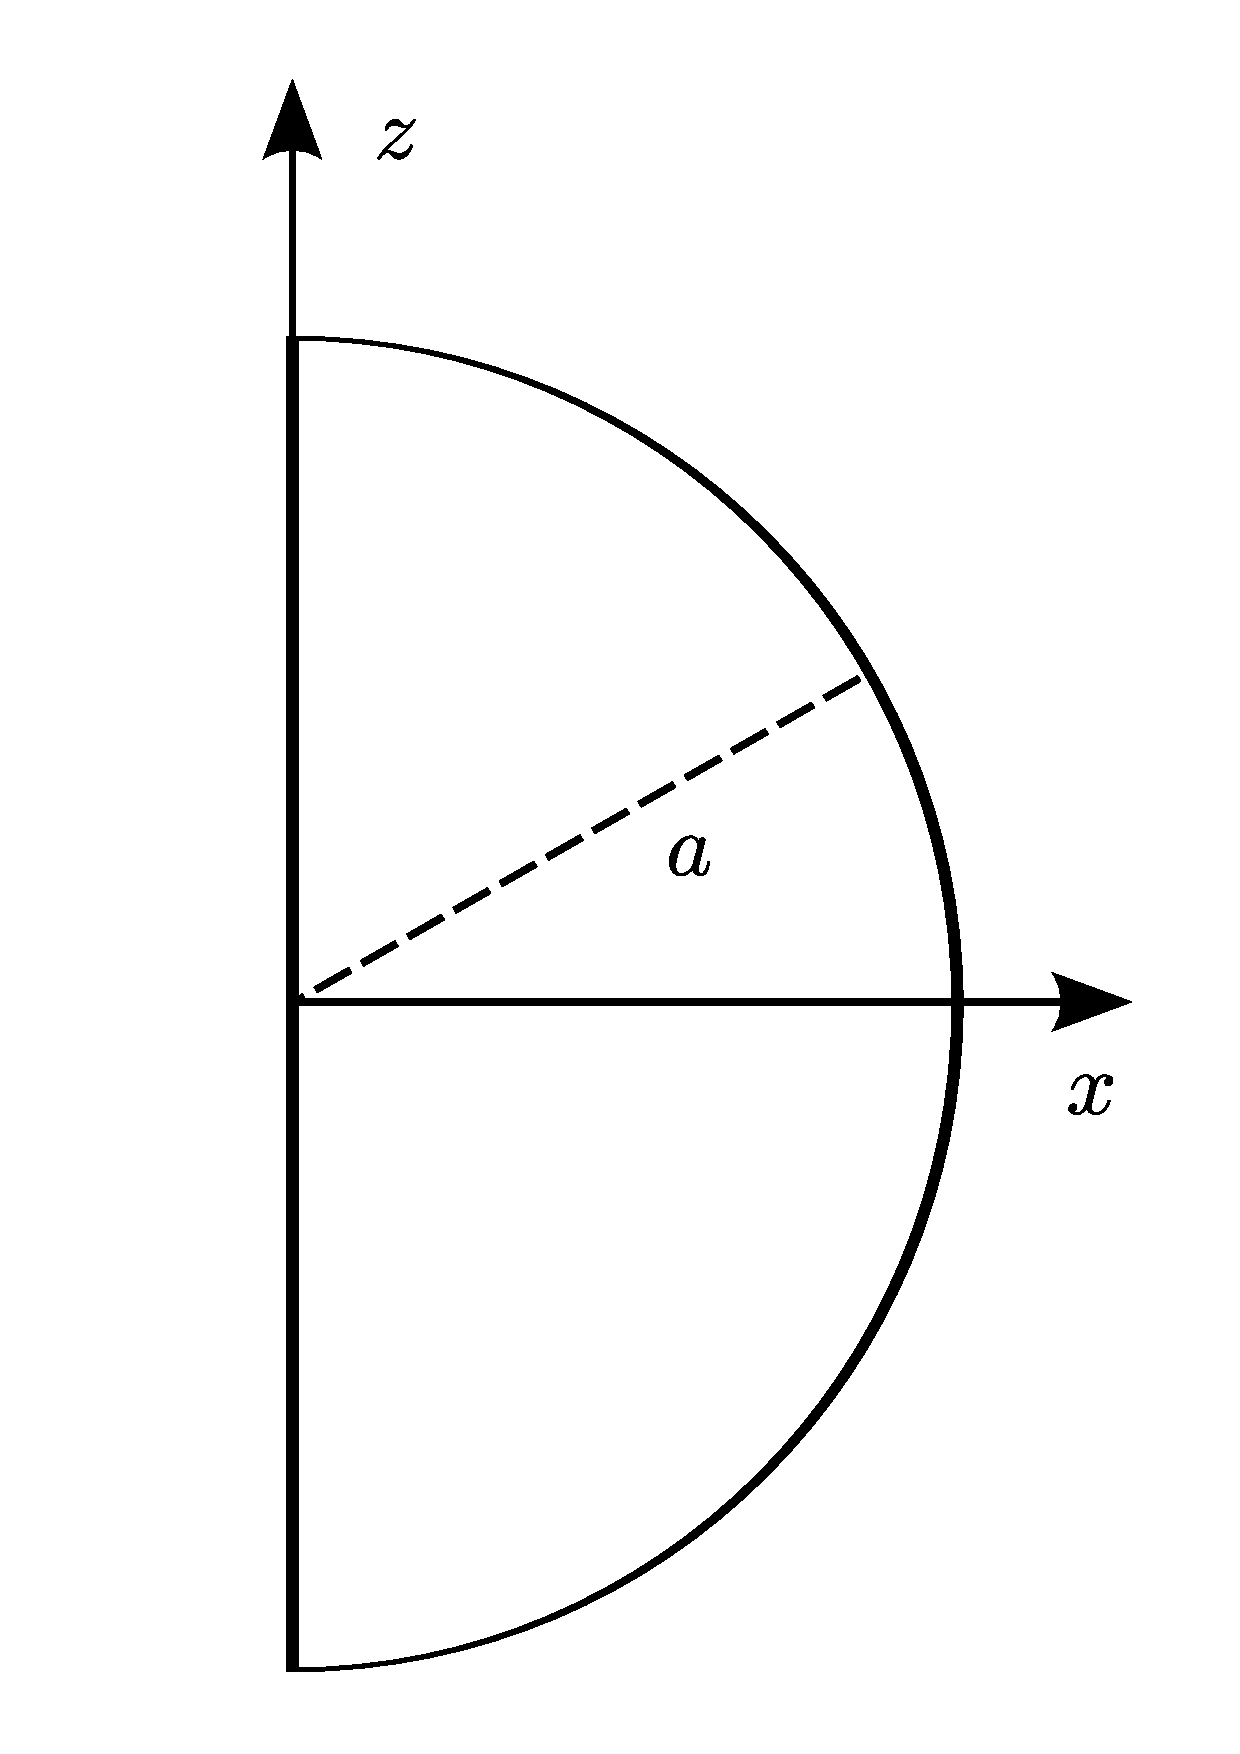
\includegraphics[width=0.95\paperwidth,height=1\paperheight, angle=0]{1.pdf}} 
%\end{figure} 

\vspace{6mm}\hspace{-14mm} 
\large \textbf{Stage de Master 2 Recherche}, \textsl{20 février 2013 - 20 juillet 2013}\\ 
\begin{center} 
\vspace{30mm} 
\huge \textbf{Oscillations d'une goutte \\ accrochée à un capillaire}\\ 
\Large \textbf{Approche de stabilité globale}\\ 
\vspace{1.5cm}

\begin{figure}[h!] 
\begin{center}
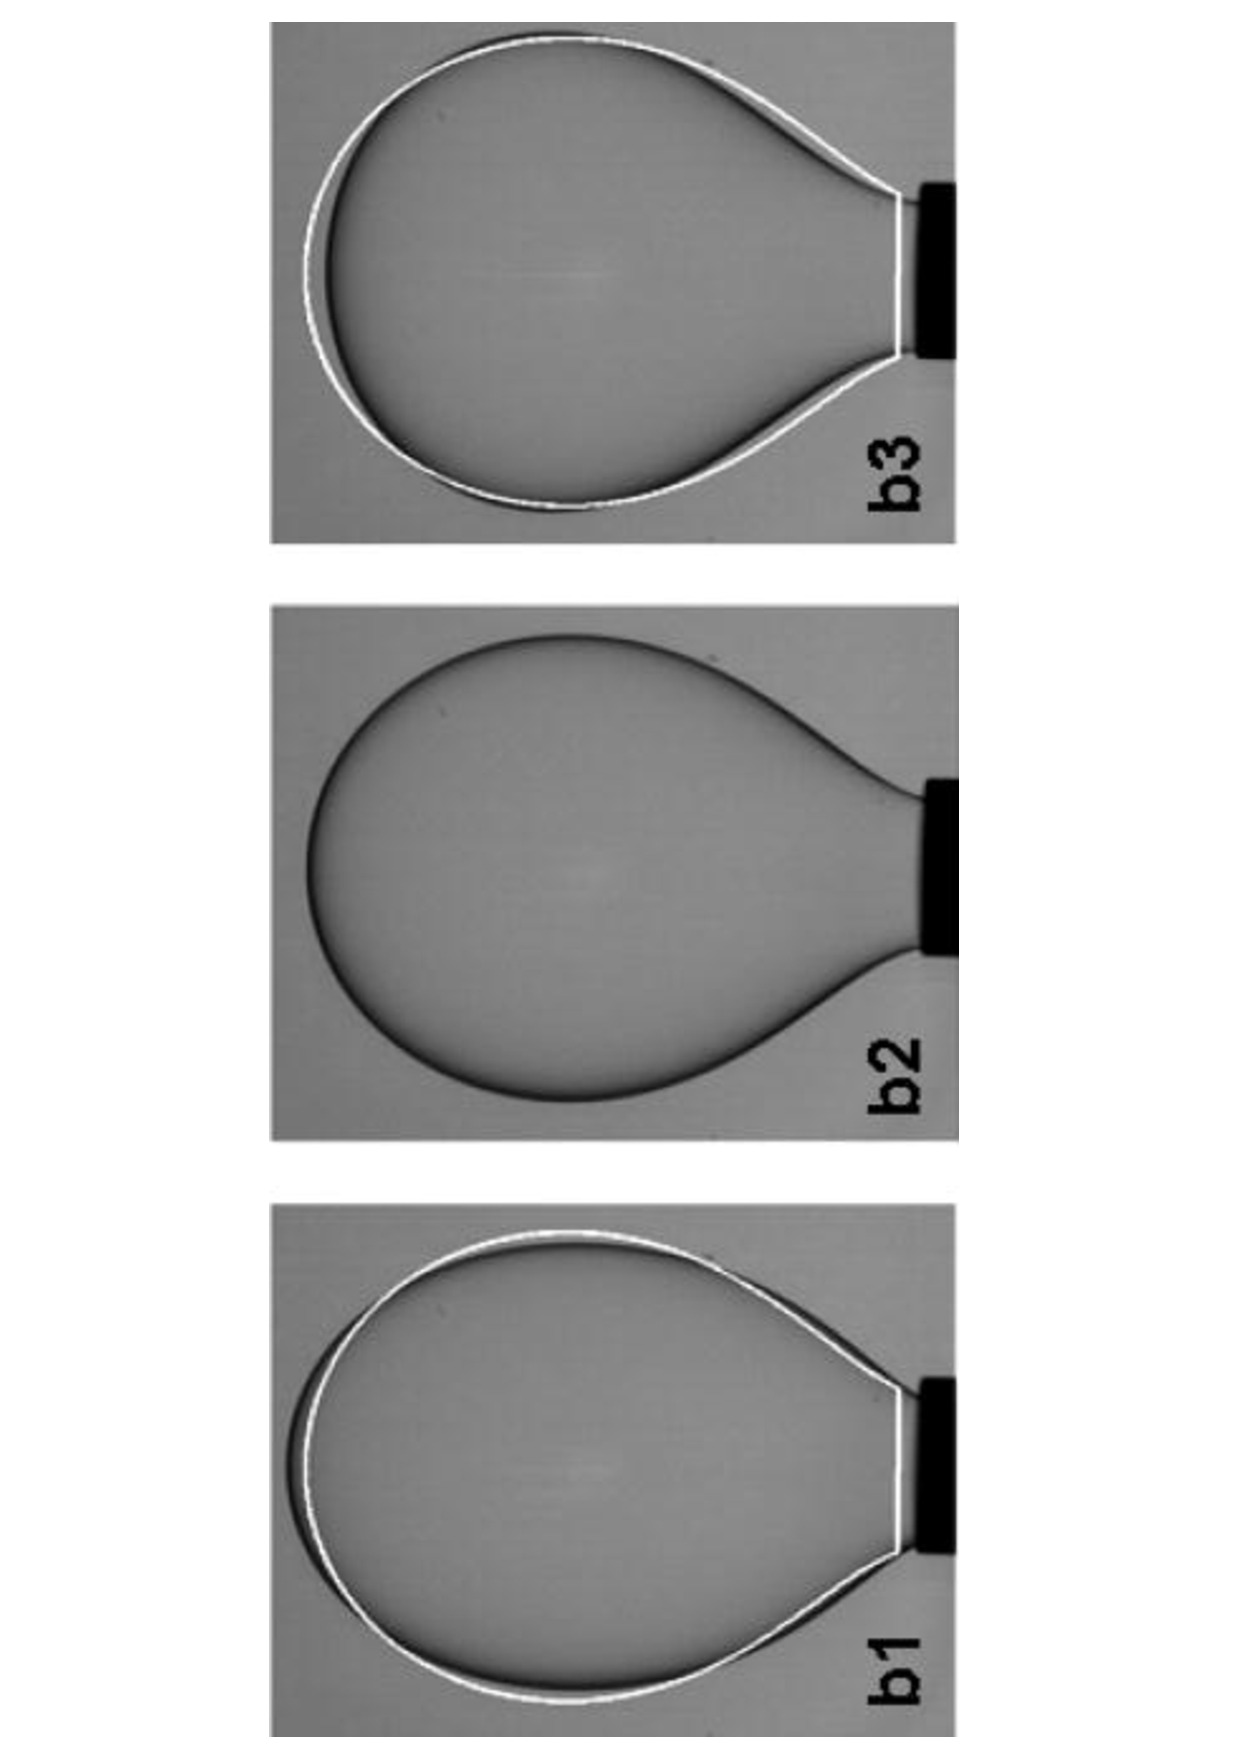
\includegraphics[width=8cm, angle=270]{title.pdf}
\end{center}
\end{figure} 

\vspace{0.3cm}
\large \textbf{Tonglei ZHANG \\} 
\textsl{Université Toulouse III - Paul Sabatier} 
 
\vspace{1cm} 
\large \textbf{MAITRE DE STAGE : \\ David FABRE}\\ 
\textsl{Institut de Mécanique des Fluides de Toulouse} 
\end{center} 

\end{titlepage}
%%%%%%%%%%%%%%%%%%%%%%%%%%%%%%%%%%%%%%%%%%%%%%%%%%%%%%%%%%%%%%%%%%%%%%%%%%%%%%%%%%%%%%%%%%%%%%%%%%%%%%%%%
%%%%%%%%%%%%%%%%%%%%%%%%%%%%%%%%%%%%%%%%%%%%%%%%%%%%%%%%%%%%%%%%%%%%%%%%%%%%%%%%%%%%%%%%%%%%%%%%%%%%%%%%%\maketitle
%\newpage
%\begin{center}
%\huge \textbf{Remerciements}
%\end{center}
%\vspace{1cm}
%\normalsize Mes premiers remerciements vont à David Fabre, 

\renewcommand\abstractname{Remerciements}

\begin{abstract}
Mes premiers remerciements vont à David Fabre, Maître de Conférence, chercheur à l'IMFT et tuteur pour mon stage de master recherche, pour m'avoir orienté tout au long de ce projet et pour m'avoir aidé dans la mise en français de ce rapport.
\\[0.25cm]
Je tiens à remercier Jérôme Mougel et Joël Tchoufag pour m'avoir aidé durant ce stage.
\\[0.25cm]
Enfin je remercie l'ensemble du groupe INTERFACE de l'IMFT, qui ont permis que ce stage se déroule dans des conditions de travail agréables.
\end{abstract}

\renewcommand\abstractname{Résumé / Abstract}

\begin{abstract}
Dans le cadre de mon stage M2R à l'IMFT, je travaille actuellement sur la stabilité d'une goutte sous la tutelle de David Fabre. Lors de ce stage, l'objectif est de mettre en place un outil permettant d'étudier les modes d'oscillation linéaires d'une goutte millimétrique d'heptane accrochée au bout d'un capillaire dans un récipient remplis d'eau. Une étude de stabilité globale sera effectuée ici en utilisant le code élément fini FreeFem++. Dans un premier temps, l'objectif sera de valider le code mis en place en se référant à des cas plus simples tel qu'une goutte sphérique en l'absence de gravité, pour laquelle existe une solution analytique. Ensuite nous nous concentrerons sur une goutte attachée pour laquelle la forme moyenne n'est pas sphérique mais déterminée par un équilibre entre les forces de gravité et la tension de surface.
\\[0.25cm]
\textsl{In the context of my M2R research internship at the IMFT, I am currently working on the stability of a drop under the guidance of David Fabre. During this internship, the objective is to establish a tool to study the linear oscillation modes of a millimetric heptane drop attached at the end of the capillary in a water-filled container. A study of global stability will be performed by using the finite element code FreeFem++. As a first step, the objective will be to validate the code established by referring to the simpler cases such as a spherical drop in the absence of gravity, for which exists an analytical solution. Afterwards we will focus on an attached drop for which the average shape is not spherical but determined by a balance between the forces of gravity and surface tension.}
\tableofcontents
\end{abstract}
%%%%%%%%%%%%%%%%%%%%%%%%%%%%%%%%%%%%%%%%%%%%%%%%%%%%%%%%%%%%%%%%%%%%%%%%%%%%%%%%%%%%%%%%%%%%%%%%%%%%%%%%%
%%%%%%%%%%%%%%%%%%%%%%%%%%%%%%%%%%%%%%%%%%%%%%%%%%%%%%%%%%%%%%%%%%%%%%%%%%%%%%%%%%%%%%%%%%%%%%%%%%%%%%%%%
%%%%%%%%%%%%%%%%%%%%%%%%%%%%%%%%%%%%%%%%%%%%%%%%%%%%%%%%%%%%%%%%%%%%%%%%%%%%%%%%%%%%%%%%%%%%%%%%%%%%%%%%%
\chapter{Introduction}
%%%%%%%%%%%%%%%%%%%%%%%%%%%%%%%%%%%%%%%%%%%%%%%%%%%%%%%%%%%%%%%%%%%%%%%%%%%%%%%%%%%%%%%%%%%%%%%%%%%%%%%%%
\section{Contexte général}
L'étude du comportement dynamique des milieux multiphasique est un des axes phares du groupe INTERFACE de l'IMFT.
À ce titre ils mènent diverses activités expérimentales et numériques visant à caractériser le comportement d'une goutte ou bulle en raison des nombreuses applications.
Une récente étude expérimentale (Figure \ref{title}) a considéré le cas d'une goutte millimétrique d'heptane accrochée au bout d'un capillaire dans un récipient rempli d'eau. Une étude fine des modes d'oscillations en régime forcé a été menée.
\begin{figure}[h!] 
\begin{center}
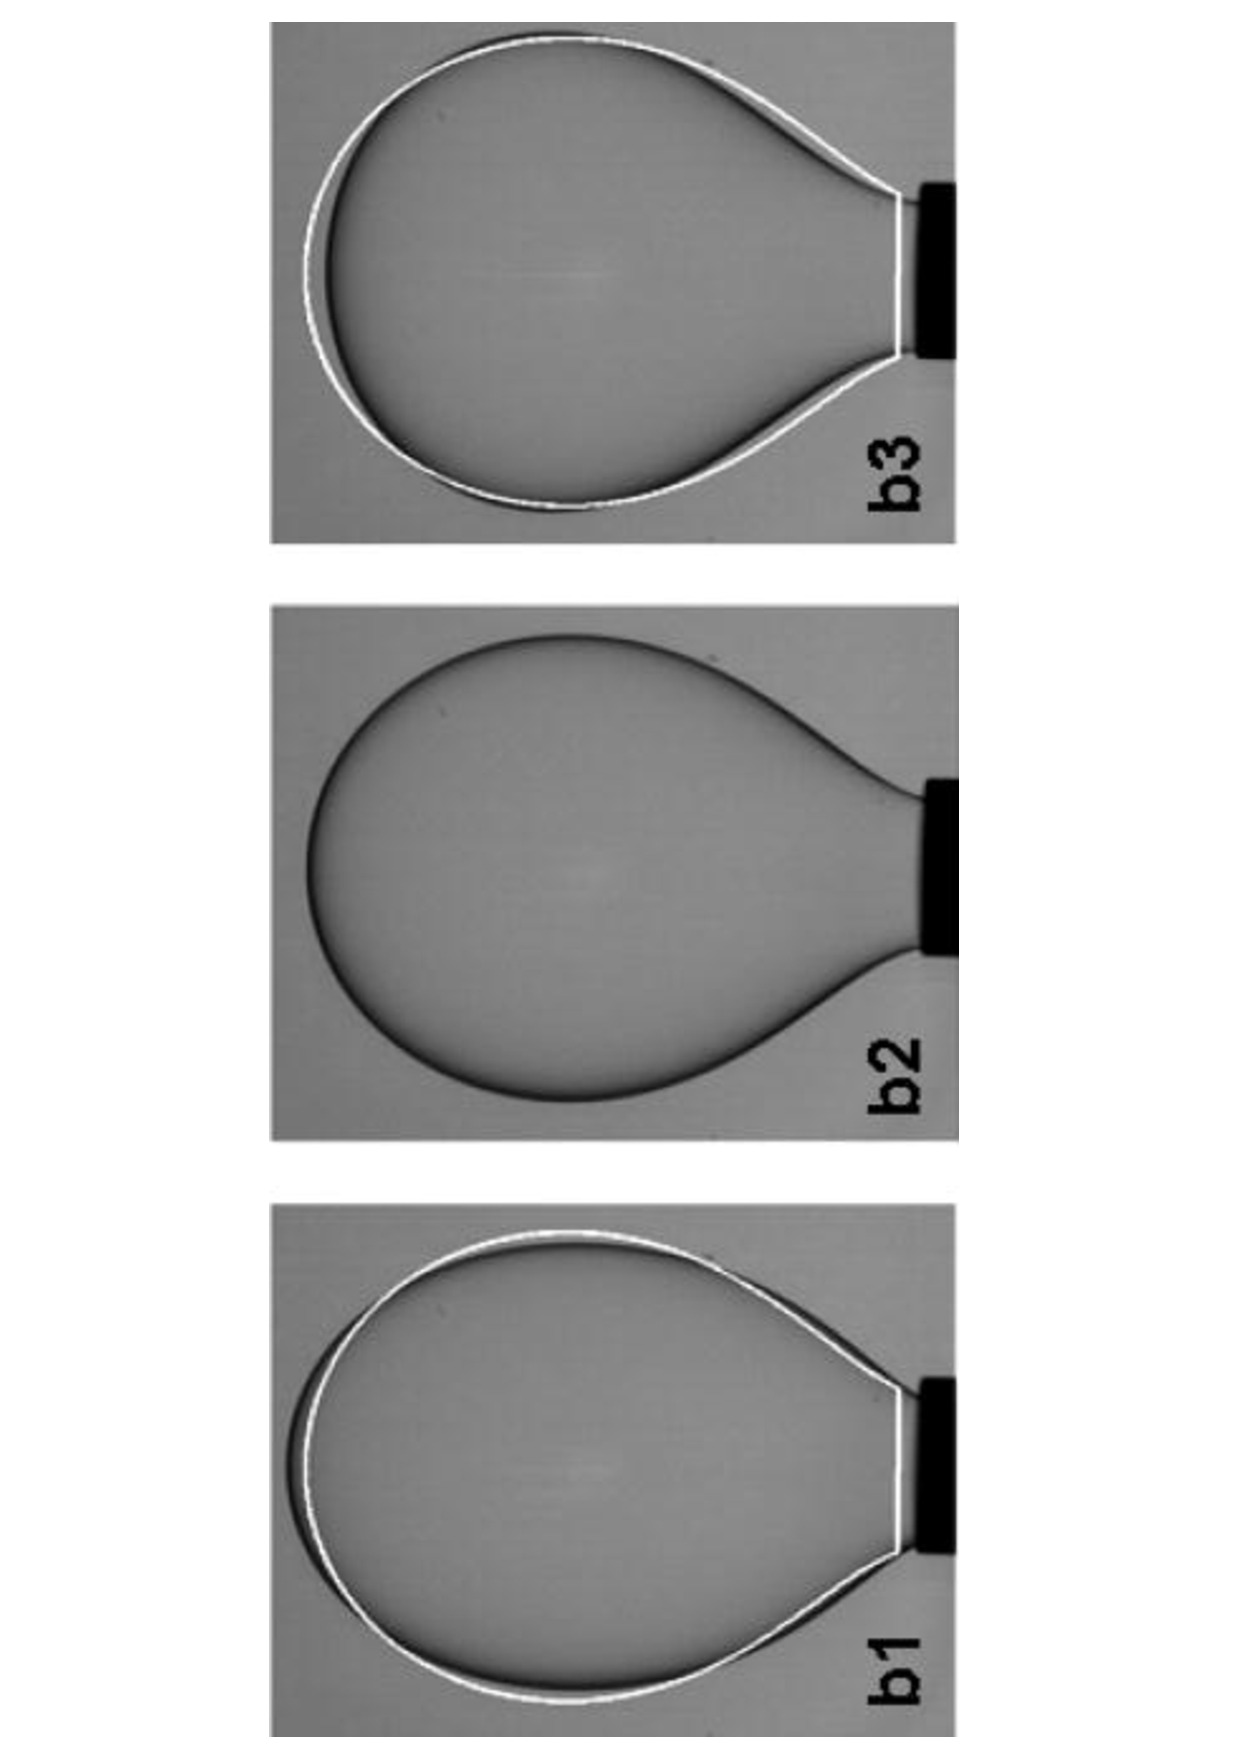
\includegraphics[width=8cm, angle=270]{title.pdf}
\caption{Oscillation d'une goutte attachée à un tube capillaire ( trois instants du cycle d'oscillation; la position moyenne est en trait blanc), N. Abi Chebel \textsl{et al} \cite{3}.}
\label{title}
\end{center}
\end{figure} 
%%%%%%%%%%%%%%%%%%%%%%%%%%%%%%%%%%%%%%%%%%%%%%%%%%%%%%%%%%%%%%%%%%%%%%%%%%%%%%%%%%%%%%%%%%%%%%%%%%%%%%%%%
\newpage
\section{Étude bibliographique}
\subsection{Modes d'une goutte libre}
D'après la théorie linéaire, Rayleigh \cite{1} a calculé les modes de vibration pour une goutte non visqueux dans le vide en l'absence de gravité. La théorie est généralisé par H. Lamb dans son livre \emph{Hydrodynamics} en 1895 \cite{2} pour les cas de Goutte ou bulle dans le milieu liquide. La théorie Rayleigh-Lamb utilise la théorie d'écoulement potentiel. La dérivation d'écoulement potentiel utilise la harmonique sphérique $Y_{n,m}$ pour décrire le comportement oscillatoire de l'interface. Dans les coordonnées sphériques $(r,\theta,\phi)$ la forme de l'interface est donnée par
\begin{eqnarray}
r = a\ [\ 1 + A_{n,m}\ Y_{n,m}(\theta,\phi)\ \cos(\omega_n t)\ ]
\end{eqnarray}
où $a$ est le rayon d'équilibre de la goutte et $A_{n,m}$ est l'amplitude du mode $(n,m)$. La fréquence propre correspondant dans le fluides diphasique est donnée par
\begin{eqnarray}
{\omega_n}^2 = \frac{ (n-1) n (n+1) (n+2) \sigma }{ ( \rho_{in} (n+1) + \rho_{ex} n ) a^3 }
\end{eqnarray}
où $\sigma$ est le coefficient de tension superficielle, $\rho_{ex}$ et $\rho_{in}$ sont les masses volumiques du fluide extérieur et du fluide intérieur respectivement.
\\[0.25cm]
On ne s'intéressera qu'aux modes axisymétriques $(m = 0)$.
\subsection{Modes d'une goutte sphérique avec contrainte}
Les études plus récentes par rapport à la théorie d'écoulement potentiel se focalisent le cas d'une goutte avec contrainte. Il est étude par A. Prosperetti \cite{4} théoriquement. Il a trouvé les modes analytique dans le cas d'une goutte qui oscille tout en étant tenue par un anneau circulaire (Figure \ref{prosperetti}) :
\begin{figure}[h!] 
\begin{center}
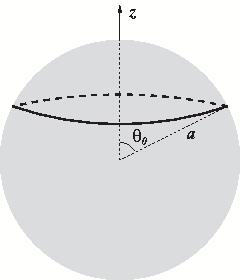
\includegraphics[width=5cm]{2_3_2_prosperetti}
\caption{Une goutte de rayon a le mouvement radial le mouvement radial duquel est prévenu par le contraint circulaire rigide}
\label{prosperetti}
\end{center}
\end{figure}
\newpage
Ses résultats sont visualisés comme la figure \ref{contrainte_Prosperetti}
\begin{figure}[h!] 
\begin{center}
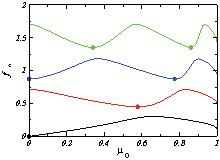
\includegraphics[width=8cm]{2_3_2_contrainte_Prosperetti.jpeg}
\caption{Les lignes sont, dans l'ordre ascendant, pour modes d'ordre n = 1, 2, 3, et 4.}
\label{contrainte_Prosperetti}
\end{center}
\end{figure}
\\
où les points remarquent les positions de la fréquence mode normal de la goutte\\
et $\mu_0 = cos(\theta_0)$, $f_* = \frac{1}{2 \pi } \sqrt{\frac{\rho a^3}{\sigma}} \omega$
\subsection{Modes d'une goutte attachée à un tube capillaire}
Le cas d'une goutte attachée à un tube capillaire est étudié expérimental par N. Abi Chebel, F. Risso et O. Masbernat \cite{3}.
Ils ont étudié les modes de la goutte par la résonance provoquée par un forçage (Figure \ref{experience}).
Ils ont trouvé que les modes d'une goutte attachée,
pour laquelle la forme moyenne n'est pas sphérique mais déterminée par un équilibre entre les forces de gravité et la tension de surface,
sont équivalent aux les modes d'une goutte libre.
\begin{figure}[h!] 
\begin{center}
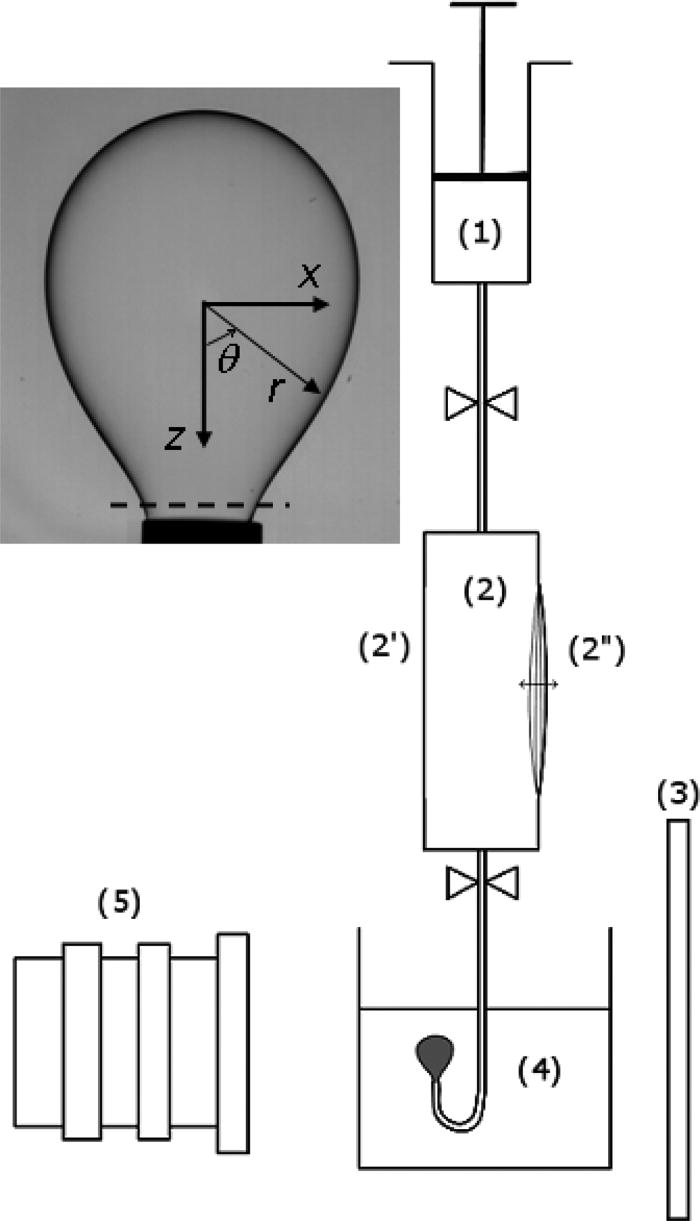
\includegraphics[width=8cm]{experience.jpg}
\caption{(2") membrane piézoélectrique}
\label{experience}
\end{center}
\end{figure}
\newpage
\section{But du stage}
Il existe des théories basées sur une décomposition en harmoniques sphériques, qui ne fonctionnent que dans le cas d'une géométrie sphérique et ne permettent donc pas de prendre en compte la déformation d'une goutte sous l'effet de la gravité.
Le but de ce travail est de mettre en place un code de calcul numérique, basé sur une méthode d'éléments finis, qui permet de traiter des formes de gouttes plus réaliste.
Le code sera tout d'abord validé par géométries sphériques dans les chapitres 2 et 3.
Puis dans le chapitre 4, on applique le code à une situation correspondante aux expériences de N. Abi Chebel, F. Risso et O. Masbernat \cite{3}, et les résultats seront comparé avec les expériences.
%%%%%%%%%%%%%%%%%%%%%%%%%%%%%%%%%%%%%%%%%%%%%%%%%%%%%%%%%%%%%%%%%%%%%%%%%%%%%%%%%%%%%%%%%%%%%%%%%%%%%%%%%
%%%%%%%%%%%%%%%%%%%%%%%%%%%%%%%%%%%%%%%%%%%%%%%%%%%%%%%%%%%%%%%%%%%%%%%%%%%%%%%%%%%%%%%%%%%%%%%%%%%%%%%%%
%%%%%%%%%%%%%%%%%%%%%%%%%%%%%%%%%%%%%%%%%%%%%%%%%%%%%%%%%%%%%%%%%%%%%%%%%%%%%%%%%%%%%%%%%%%%%%%%%%%%%%%%%
\chapter{Goutte ou bulle non visqueux}
%%%%%%%%%%%%%%%%%%%%%%%%%%%%%%%%%%%%%%%%%%%%%%%%%%%%%%%%%%%%%%%%%%%%%%%%%%%%%%%%%%%%%%%%%%%%%%%%%%%%%%%%%
\section{Position du problème}
%%%%%%%%%%%%%%%%%%%%%%%%%%%%%%%%%%%%%%%%%%%%%%%%%%%%
\begin{figure}[!htbp]
\centering
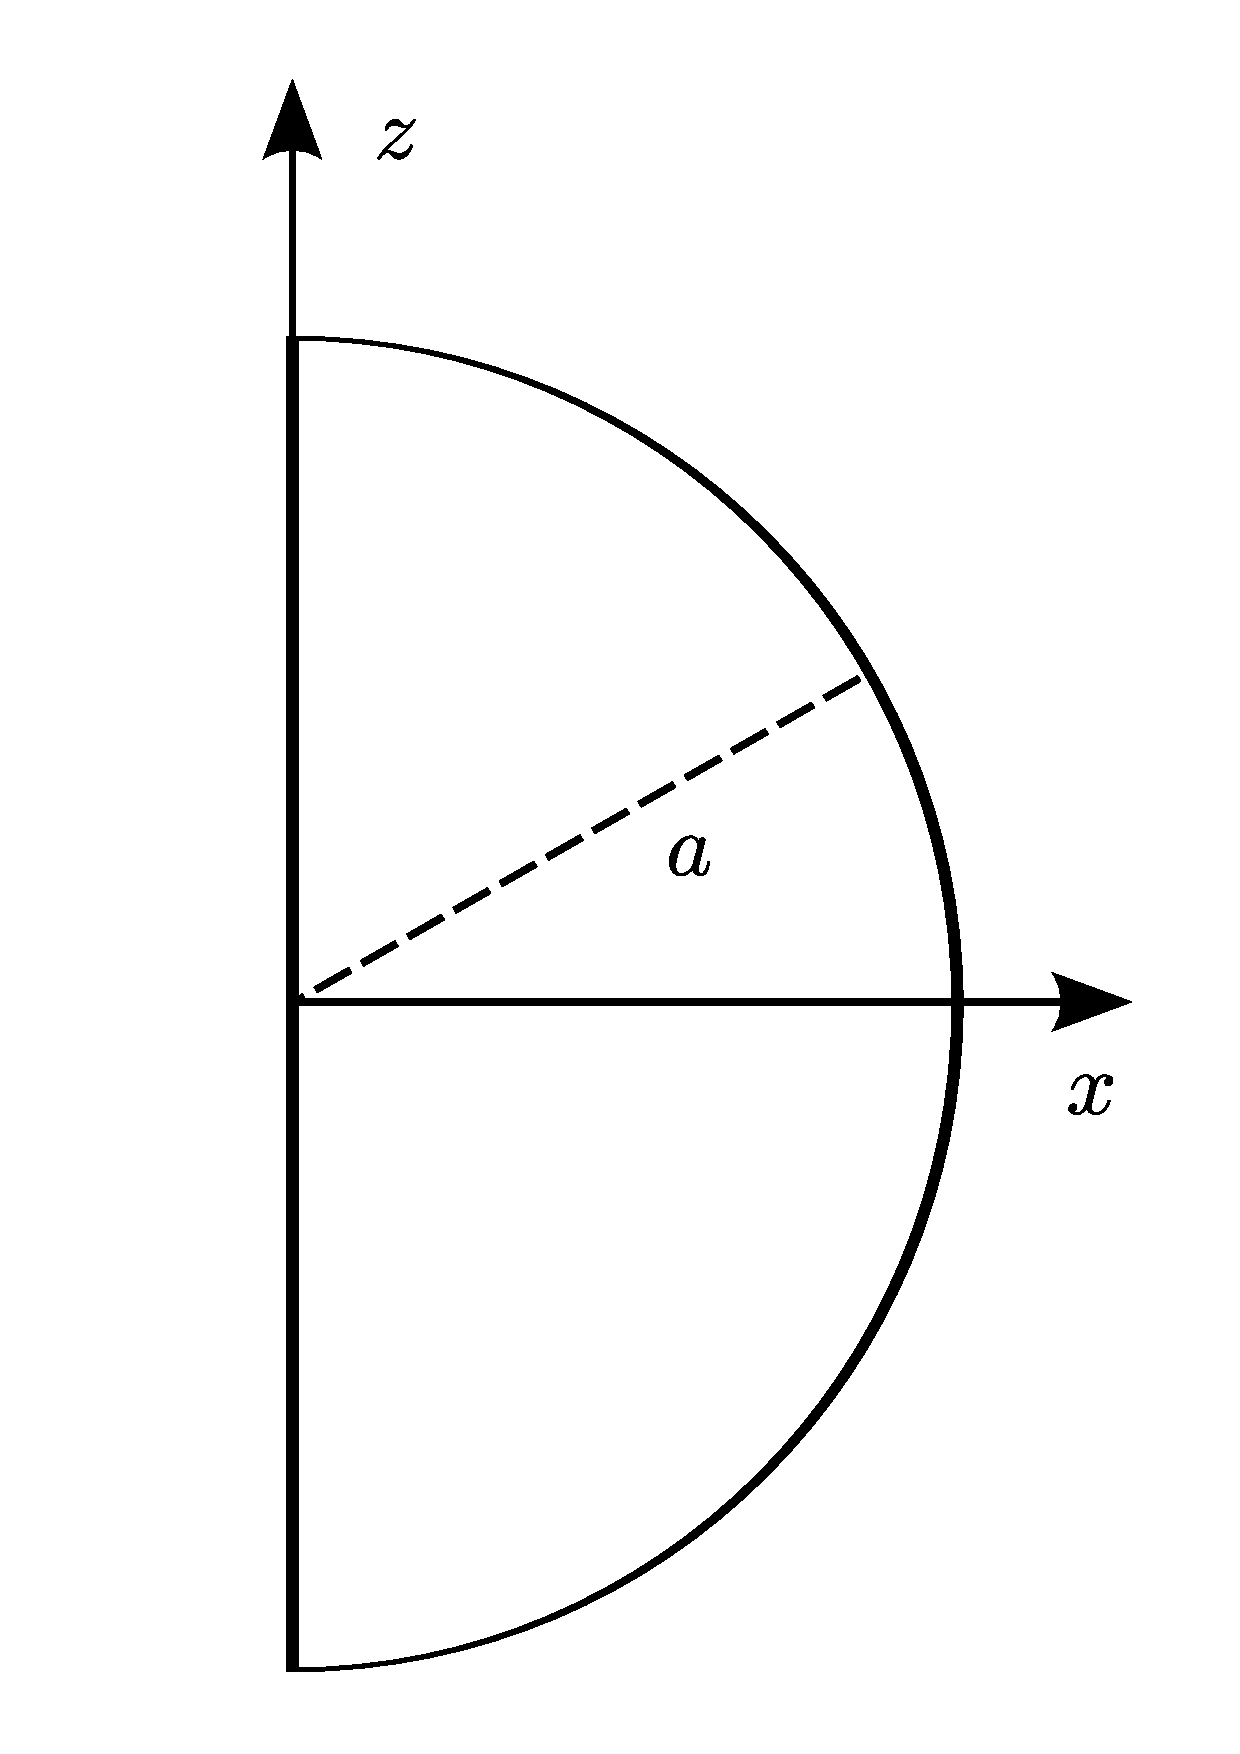
\includegraphics[width=4cm]{1.pdf}
\caption{La champ de base pour une goutte}
%\label{fig_res}
\end{figure}
Nous adopterons le système de coordonnées sphériques $(r,\theta,\phi)$ centré au centre de la goutte.
\begin{tabbing}
Notons :\\
$a$\,\    \= : le rayon d'équilibre de la goutte\\
$\varPhi$ \> : le potentiel de vitesse\\
$P$       \> : la pression du côté intérieur\\
$H$       \> : le rayon de la goutte
\end{tabbing}
%%%%%%%%%%%%%%%%%%%%%%%%%%%%%%%%%%%%%%%%%%%%%%%%%%%%
\subsection{Équations générales}
\begin{eqnarray}\label{pb:1}         %方程组开始
\left\{                              %方程组的左边包括大括号\{
\begin{array}{lll}                   %设定列阵的格式:{lll}是三个L,表示三列的对齐方式为Left对齐
\Delta \varPhi = 0                                                                                     & \text{dans le volume $\Omega$}    \\%&——分隔列的标记,\\——表示换行
P + \rho\ \frac{\partial}{\partial t}\varPhi = 0                                                        & \text{dans le volume $\Omega$}    \\%&同上
\frac{\partial}{\partial t} H = \nabla \varPhi \cdot \vec{n} = \frac{\partial}{\partial r} \varPhi     & \text{sur la surface libre $S$ (Condition cinématique)}      \\
P = \sigma\ \mathscr{C}                              & \text{sur la surface libre $S$ (Condition dynamique)}   % \mathcal{C} ou \mathscr{C}
\end{array}                          %方程列阵的结束
\right.                              %方程组的右边无符号,利用“.“来标示
\end{eqnarray}                       %方程组结束
\begin{flalign*}
\text{où}   & &\\
\rho        &: \text{la masse volumique du fluide} &\\
\sigma      &: \text{le coefficient de tension superficielle} &\\
\mathscr{C} &: \text{la courbure moyenne de l'interface} &
\end{flalign*}
%%%%%%%%%%%%%%%%%%%%%%%%%%%%%%%%%%%%%%%%%%%%%%%%%%%%
\subsection{Décomposition modale}
On considère maintenant l'oscillation linéaire d'une goutte sphérique par rapport à la position d'équilibre :
\begin{eqnarray*}
\varPhi &=& \varPhi_0 + \varphi(r,\theta,\phi)\ e^{- i \omega t} \\
P       &=& P_0 + p(r,\theta,\phi)\ e^{- i \omega t}\\
H       &=& a + \varepsilon\ \eta(\theta,\phi)\ e^{- i \omega t}
\end{eqnarray*}
Nous exprimons la forme de la goutte comme une fonction implicite $S_d$ telle que :
\begin{eqnarray}
S_d(r,\theta,\phi,t) = r - [\ a + \varepsilon\ \eta(\theta,\phi)\ e^{- i \omega t}\ ] = 0.
\end{eqnarray}
où $\varepsilon$ est un petit paramètre.
\\[0.25cm]
Pour une courbe plane représentée sous la forme de fonction implicite $S_d(r,\theta,\phi,t) = 0$, on sait que
la courbure est définie comme :
\begin{eqnarray*}
\mathscr{C} = div(\vec{n}) \qquad \text{où} \ \vec{n} = \frac{\nabla S_d}{\Vert \nabla S_d \Vert}
\end{eqnarray*}
La courbure de la surface libre se calcule alors de la façon suivant :
\begin{flalign*}
\nabla S_d &= \frac{\partial}{\partial r} S_d \ \boldsymbol{e_r}
              + \left[\ \frac{1}{r} \frac{\partial}{\partial \theta} S_d \ \boldsymbol{e_\theta}
                        + \frac{1}{r \sin\theta} \frac{\partial}{\partial \phi} S_d \ \boldsymbol{e_\phi}\ \right]\ e^{- i \omega t}&\\ % \boldsymbol{e_\phi} ou \pmb{e_\phi}
           &= 1 \ \boldsymbol{e_r}
              - \varepsilon \left[\ \frac{1}{r} \frac{\partial}{\partial \theta} \eta \ \boldsymbol{e_\theta}
                                    + \frac{1}{r \sin\theta} \frac{\partial}{\partial \phi} \eta \ \boldsymbol{e_\phi}\ \right]\ e^{- i \omega t}&
\end{flalign*}
\begin{flalign*}
\Vert \nabla S_d \Vert &= \left \| \ 1 \ \boldsymbol{e_r}
                                     - \varepsilon \left[\ \frac{1}{r} \frac{\partial}{\partial \theta} \eta \ \boldsymbol{e_\theta}
                                     + \frac{1}{r \sin\theta} \frac{\partial}{\partial \phi} \eta \ \boldsymbol{e_\phi}\ \right]\ e^{- i \omega t}\ \right \| &\\
                       &= \sqrt{ 1 + o(\varepsilon^2) } &\\
                       &= 1 + o(\varepsilon^2)&
\end{flalign*}
\begin{flalign*}
\vec{n} &= 1 \ \boldsymbol{e_r}
           - \varepsilon \left[\ \frac{1}{r} \frac{\partial}{\partial \theta} \eta \ \boldsymbol{e_\theta}
                                 + \frac{1}{r \sin\theta} \frac{\partial}{\partial \phi} \eta \ \boldsymbol{e_\phi}\ \right]\ e^{- i \omega t}
           + o(\varepsilon^2)&
\end{flalign*}
\begin{flalign*}
div(\vec{n}) &= \frac{1}{r^2} \frac{\partial}{\partial r}[\ r^2 \ 1 \ ]
                + \varepsilon \left[\ \frac{1}{r \sin\theta} \frac{\partial}{\partial \theta}[\ \sin\theta \ (- \frac{1}{r} \frac{\partial}{\partial \theta} \eta) \ ]
                          + \frac{1}{r \sin\theta} \frac{\partial}{\partial \phi}[\ - \frac{1}{r \sin\theta} \frac{\partial}{\partial \phi} \eta \ ]\ \right]\ e^{- i \omega t}
                + o(\varepsilon^2)&\\
             &= \frac{2}{r}
                - \varepsilon \left[\ \frac{1}{r^2 \sin\theta} \frac{\partial}{\partial \theta}(\ \sin\theta \ \frac{\partial}{\partial \theta} \eta \ )
                           + \frac{1}{r^2 \sin\theta} \frac{\partial}{\partial \phi}(\ \frac{1}{\sin\theta} \frac{\partial}{\partial \phi} \eta \ )\ \right]\ e^{- i \omega t}
                + o(\varepsilon^2)&\\
             &= \frac{2}{r}
                - \varepsilon \frac{1}{r^2 \sin\theta} \left[\ \frac{\partial}{\partial \theta}(\ \sin\theta \ \frac{\partial}{\partial \theta} \eta \ )
                                               + \frac{\partial}{\partial \phi}(\ \frac{1}{\sin\theta} \frac{\partial}{\partial \phi} \eta \ )\ \right]\ e^{- i \omega t}
                + o(\varepsilon^2)&
\end{flalign*}
on remplace $r$ par $\left[\ a + \varepsilon \ \eta \ e^{- i \omega t}\ \right]$, on a
\begin{flalign*}
\frac{1}{r}   &= \frac{1}{a + \varepsilon \ \eta \ e^{- i \omega t}}
               = \frac{1}{a} - \varepsilon \ \frac{1}{a^2} \ \eta \ e^{- i \omega t} + o(\varepsilon^2)&\\
\frac{1}{r^2} &= \frac{1}{a^2} + o(\varepsilon^2)&
\end{flalign*}
alors
\begin{flalign*}
\mathscr{C} &= div(\vec{n})&\\
            &= \frac{2}{a} - \varepsilon \frac{2}{a^2} \ \eta(\theta,\phi)\ e^{- i \omega t}
               - \varepsilon \frac{1}{a^2 \sin\theta} \left[\ \frac{\partial}{\partial \theta}(\ \sin\theta \ \frac{\partial}{\partial \theta} \eta \ )
                                                    + \frac{\partial}{\partial \phi}(\ \frac{1}{\sin\theta} \frac{\partial}{\partial \phi} \eta \ )\ \right]\ e^{- i \omega t}
               + o(\varepsilon^2)&\\
            &= \mathscr{C}_0 + \varepsilon \ \mathscr{C}_1 + o(\varepsilon^2)&
\end{flalign*}
On obtient ainsi le terme de courbure lié aux petites perturbations :
\begin{eqnarray}
\mathscr{C}_1 = - \frac{2}{a^2} \ \eta \ e^{- i \omega t}
                - \frac{1}{a^2 \sin\theta} \left[\ \frac{\partial}{\partial \theta}(\ \sin\theta \ \frac{\partial}{\partial \theta} \eta \ )
                                                    + \frac{\partial}{\partial \phi}(\ \frac{1}{\sin\theta} \frac{\partial}{\partial \phi} \eta \ )\ \right]\ e^{- i \omega t}
\end{eqnarray}
dans le cadre de ce sujet, on met $\phi = 0$, alors
\begin{eqnarray}
\mathscr{C}_1 = - \left[\ \frac{2}{a^2} \ \eta
                          + \frac{1}{a^2 \sin\theta} \frac{\partial}{\partial \theta}(\ \sin\theta \ \frac{\partial}{\partial \theta} \eta \ )\ \right]\ e^{- i \omega t}.
\end{eqnarray}
%%%%%%%%%%%%%%%%%%%%%%%%%%%%%%%%%%%%%%%%%%%%%%%%%%%%
\subsection{Linéarisation des équations}
La linéarisation des équations s'effectue en remplaçant dans le système d'équations d'équilibre \eqref{pb:1} le potentiel de vitesse, le champ de pression et la courbure par leur décomposition, puis en conservant uniquement les termes d'ordre 1 par rapport aux petites perturbation introduites. Nous obtenons ainsi le problème linéaire suivant :
\begin{eqnarray}\label{pb:2}         %方程组开始
\left\{                              %方程组的左边包括大括号\{
\begin{array}{lll}                   %设定列阵的格式:{lll}是三个L,表示三列的对齐方式为Left对齐
\Delta \varphi = 0                                                                                     & \text{dans le volume $\Omega$}    \\%&——分隔列的标记,\\——表示换行
p + \lambda\ \rho\ \varphi = 0                                                        & \text{dans le volume $\Omega$}    \\%&同上
\lambda\ \eta = \nabla \varphi \cdot \vec{n} = \frac{\partial}{\partial r} \varphi     & \text{sur la surface libre $S$ (Condition cinématique)}      \\
p = - \sigma\ \left[\ \frac{2}{a^2} \ \eta
                      + \frac{1}{a^2 \sin\theta} \frac{\partial}{\partial \theta}(\ \sin\theta \ \frac{\partial}{\partial \theta} \eta \ )\ \right]
& \text{sur la surface libre $S$ (Condition dynamique)}   % \mathcal{C} ou \mathscr{C}
\end{array}                          %方程列阵的结束
\right.                              %方程组的右边无符号,利用“.“来标示
\end{eqnarray}                       %方程组结束
Avec $\lambda = - i \omega t$ les valeurs propre recherchés.
%%%%%%%%%%%%%%%%%%%%%%%%%%%%%%%%%%%%%%%%%%%%%%%%%%%%%%%%%%%%%%%%%%%%%%%%%%%%%%%%%%%%%%%%%%%%%%%%%%%%%%%%%
\section{Modélisation numérique}
%%%%%%%%%%%%%%%%%%%%%%%%%%%%%%%%%%%%%%%%%%%%%%%%%%%%
\subsection{Formulation variationnelle}
Pour l'implémentation de ces équations sous FreeFem++ il convient de mettre en place une formulation variationnelle (ou formulation faible). Pour cela, introduit des fonction test $(\varphi^*, p^*, \eta^*)$ associées à $(\varphi, p, \eta)$.
\\[0.25cm]
La formulation variationnelle du problème \eqref{pb:2} se met alors en plusieurs étapes. Dans un premiers temps, on multiplie scalairement les équation du problème \eqref{pb:2} par leur fonction test associée :
\\[0.25cm]
$\forall (\varphi^*, p^*, \eta^*)$,
\begin{eqnarray*}
\left\{
\begin{array}{rcl}
\left(\ \Delta \varphi\ \right) \cdot \varphi^* &=& 0 \\
\left(\ p + \lambda\ \rho\ \varphi\ \right) \cdot p^* &=& 0 \\
\left(\ p + \sigma\ \left[\ \frac{2}{a^2} \ \eta
                    + \frac{1}{a^2 \sin\theta} \frac{\partial}{\partial \theta}(\ \sin\theta \ \frac{\partial}{\partial \theta} \eta \ )\ \right]\ \right) \cdot \eta^* &=& 0
\end{array}
\right.
\end{eqnarray*}
Ensuite, on intègres ces trois équations. On obtient alors :
\\[0.25cm]
$\forall (\varphi^*, p^*, \eta^*)$,
\begin{eqnarray*}
\left\{
\begin{array}{rcl}
(\ \Delta \varphi ,\ \varphi^* \ )_\Omega &=& 0 \\
(\ - p ,\ p^* \ )_\Omega &=& \lambda\ (\ \rho\ \varphi ,\ p^* \ )_\Omega \\
<\ p + \sigma\ \left[\ \frac{2}{a^2} \ \eta
                       + \frac{1}{a^2 \sin\theta} \frac{\partial}{\partial \theta}(\ \sin\theta \ \frac{\partial}{\partial \theta} \eta \ )\ \right] ,\ \eta^* \ >_S &=& 0
\end{array}
\right.
\end{eqnarray*}
Enfin, la condition cinématique est introduite au sein de cette formulation grâce à la formule de Green s'écrit :
\\[0.25cm]
$\forall \varphi^*$,
\begin{eqnarray*}
(\ \Delta \varphi ,\ \varphi^* \ )_\Omega = - (\ \nabla \varphi ,\ \nabla \varphi^* \ )_\Omega + <\ \nabla \varphi \cdot \vec{n},\ \varphi^* \ >_S
\end{eqnarray*}
Or la condition cinématique donne $\lambda\ a\ \eta = \nabla \varphi \cdot \vec{n} = \frac{\partial}{\partial r} \varphi$. On obtient donc :
\\[0.25cm]
$\forall \varphi^*$,
\begin{eqnarray*}
(\ \Delta \varphi ,\ \varphi^* \ )_\Omega = - (\ \nabla \varphi ,\ \nabla \varphi^* \ )_\Omega + \lambda\ <\ \eta,\ \varphi^* \ >_S
\end{eqnarray*}
On en déduit alors la formulation faible du problème \eqref{pb:2} :
\\[0.25cm]
$\forall (\varphi^*, p^*, \eta^*)$,
\begin{eqnarray}\label{pb:3}
\left\{
\begin{array}{rcl}
(\ \nabla \varphi ,\ \nabla \varphi^* \ )_\Omega &=& \lambda\ <\ \eta,\ \varphi^* \ >_S \\
- (\ p ,\ p^* \ )_\Omega &=& \lambda\ (\ \rho\ \varphi ,\ p^* \ )_\Omega \\
<\ p + \sigma\ \left[\ \frac{2}{a^2} \ \eta
                       + \frac{1}{a^2 \sin\theta} \frac{\partial}{\partial \theta}(\ \sin\theta \ \frac{\partial}{\partial \theta} \eta \ )\ \right] ,\ \eta^* \ >_S &=& 0
\end{array}
\right.
\end{eqnarray}
On trouve que
\begin{eqnarray*}
<\ \sigma\ \frac{1}{a^2 \sin\theta} \frac{\partial}{\partial \theta}(\ \sin\theta \ \frac{\partial}{\partial \theta} \eta \ ) ,\ \eta^* \ >_S
=
- <\ \sigma\ \frac{1}{a^2} \frac{\partial}{\partial \theta} \eta ,\ \frac{\partial}{\partial \theta} \eta* \ >_S
\end{eqnarray*}
On peux simplifie la formulation \eqref{pb:3} comme la forme suivante :
\begin{eqnarray}\label{pb:4}
\left\{
\begin{array}{rcl}
(\ \nabla \varphi ,\ \nabla \varphi^* \ )_\Omega &=& \lambda\ <\ \eta,\ \varphi^* \ >_S \\
- (\ p ,\ p^* \ )_\Omega &=& \lambda\ (\ \rho\ \varphi ,\ p^* \ )_\Omega \\
<\ p + \sigma\ \frac{2}{a^2} \ \eta ,\ \eta^* \ >_S - <\ \sigma\ \frac{1}{a^2} \frac{\partial}{\partial \theta} \eta ,\ \frac{\partial}{\partial \theta} \eta* \ >_S &=& 0
\end{array}
\right.
\end{eqnarray}
%%%%%%%%%%%%%%%%%%%%%%%%%%%%%%%%%%%%%%%%%%%%%%%%%%%%
\subsection{Écriture du problème sous forme matricielle}
On peut met la formulation variationnelle \eqref{pb:4} sous la forme matricielle suivante :
\begin{equation}\label{eq:55}
\begin{bmatrix}
A_{11} & 0      & 0 \\
0      & A_{22} & 0 \\
0      & A_{32} & A_{33}
\end{bmatrix}
=
\lambda
\begin{bmatrix}
0      & 0 & B_{13} \\
B_{21} & 0 & 0 \\
0      & 0 & 0
\end{bmatrix}
\end{equation}
Or, il s'avère que la formulation \eqref{eq:55} est singulière. On ajoute un terme pénalisation $\epsilon \eta \eta^*$ à matrice $A$ comme la forme suivant :
\begin{equation}\label{eq:5}
\begin{bmatrix}
A_{11} & 0      & 0 \\
0      & A_{22} & 0 \\
0      & A_{32} & A_{33} + \epsilon \eta \eta^*
\end{bmatrix}
=
\lambda
\begin{bmatrix}
0      & 0 & B_{13} \\
B_{21} & 0 & 0 \\
0      & 0 & 0
\end{bmatrix}
\end{equation}
%%%%%%%%%%%%%%%%%%%%%%%%%%%%%%%%%%%%%%%%%%%%%%%%%%%%%%%%%%%%%%%%%%%%%%%%%%%%%%%%%%%%%%%%%%%%%%%%%%%%%%%%%
\newpage
\section{Validation du code}
%%%%%%%%%%%%%%%%%%%%%%%%%%%%%%%%%%%%%%%%%%%%%%%%%%%%
\subsection{Cas d'une goutte sans contrainte}
On sait que la valeur propre d'une goutte non visqueux est généralisé par H. Lamb sous la forme suivante :
\begin{eqnarray*}
{\omega_n}^2 = n (n-1) (n+2) \frac{\sigma}{\rho a^3}
\end{eqnarray*}
On met $\sigma = 1$, $\rho = 1$, $a = 1$ et le parametre de pénalisation $\epsilon = 10^{-7}$ pour comparer les données dans le tableau suivant :

\begin{table}[htp]
\begin{center}
    \begin{tabular}{ | l | l | l | l | l | }
    \hline
    Mode & $\omega_2$ & $\omega_3$ & $\omega_4$ \\
    \hline
    $N = 343$   & 2.83907 & 5.52070 & 8.59330 \\ %10
    \hline
    $N = 1372$  & 2.83108 & 5.48809 & 8.51209 \\ %20
    \hline
    $N = 3114$  & 2.82957 & 5.48195 & 8.49715 \\ %30
    \hline
    $N = 5523$  & 2.82907 & 5.47985 & 8.49182 \\ %40
    \hline
    $N = 8641$  & 2.82883 & 5.47889 & 8.48943 \\ %50
    \hline
    $N = 12642$ & 2.82871 & 5.47839 & 8.48818 \\ %60
    \hline
    $N = 16861$ & 2.82863 & 5.47808 & 8.48742 \\ %70
    \hline
    $N = 22767$ & 2.82858 & 5.47788 & 8.48691 \\ %80
    \hline
    $N = 27862$ & 2.82855 & 5.47774 & 8.48657 \\ %90
    \hline
    $N = 34484$ & 2.82852 & 5.47764 & 8.48632 \\ %100
    \hline
    Théorique   & 2.82843 & 5.47723 & 8.48528 \\
    \hline
    \end{tabular}
\end{center}
    \caption{Modes deux, trois et quatre d'une goutte libre}
\end{table}










Avec $N$ le nombre de triangles constituant le maillage.
\\[0.25cm]
Nous obtenons des valeurs propres très proches de celles obtenues analytiquement par H. Lamb.
\\[0.25cm]
On choisi le troisième mode $\omega_3 = 5.47723$ pour étudier la convergence de code FreeFem++.


\begin{figure}[h!] 
\begin{center}
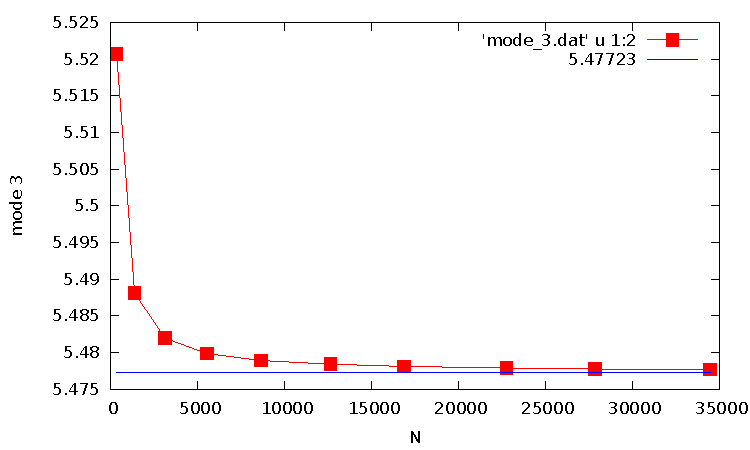
\includegraphics[width=10cm]{2_3_1_mode_3}
\caption{La convergence du nombre de triangles constituant le maillage}
%\label{experience}
\end{center}
\end{figure}

%\begin{center}
%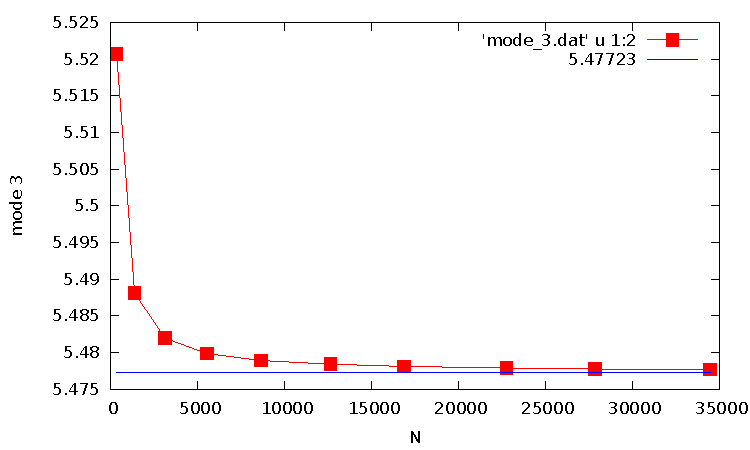
\includegraphics[width=10cm]{2_3_1_mode_3}
%\end{center}
On peut considérer que le code FreeFem++ est converge par rapport au nombre de triangles constituant le maillage.
\\[0.25cm]
Ensuite on choisi le nombre de triangles $N = 50$ pour étudier la sensibilité du parametre de pénalisation $\epsilon$.
\begin{table}[htp]
\begin{center}
    \begin{tabular}{ | l | l | l | l | l | }
    \hline
    Mode & $\omega_2$ & $\omega_3$ & $\omega_4$ \\
    \hline
    $\epsilon = 10^{-3}$  & 2.82884 & 5.47889 & 8.48943 \\
    \hline
    $\epsilon = 10^{-4}$  & 2.82883 & 5.47889 & 8.48943 \\
    \hline
    $\epsilon = 10^{-5}$  & 2.82883 & 5.47889 & 8.48943 \\
    \hline
    $\epsilon = 10^{-6}$  & 2.82883 & 5.47889 & 8.48943 \\
    \hline
    $\epsilon = 10^{-7}$  & 2.82883 & 5.47889 & 8.48943 \\
    \hline
    $\epsilon = 10^{-8}$  & nul & nul & nul \\
    \hline
    Théorique   & 2.82843 & 5.47723 & 8.48528 \\
    \hline
    \end{tabular}
\end{center}
\caption{La convergence du paramètre de pénalisation}
\end{table}

On peut considérer que la sensibilité du paramètre de pénalisation $\epsilon$ est nécessaire et son effet sur les solutions est négligeable.
\\[0.25cm]
Enfin on choisi le troisième mode $\omega_3 = 5.47723$ et le nombre de triangles $N = 8641$ pour visualiser le potentiel de vitesse, le champ de vitesse, la pression et le déplacement de surface.



\begin{figure}[h!] 
\begin{center}
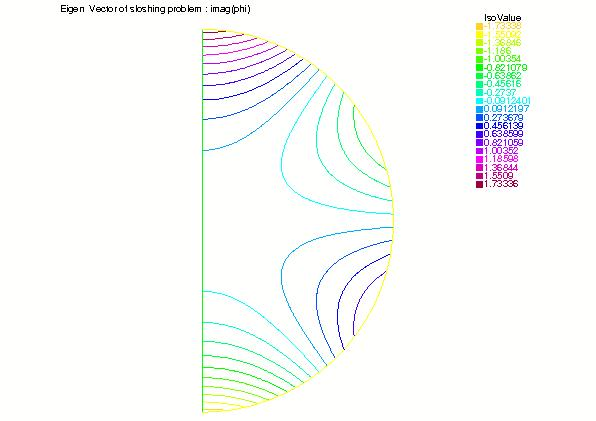
\includegraphics[width=6cm]{2_3_1_potentiel_de_vitesse.jpeg}
\caption{potentiel de vitesse}
%\label{experience}
\end{center}
\end{figure}

%\begin{figure}[!htbp]
%\centering
%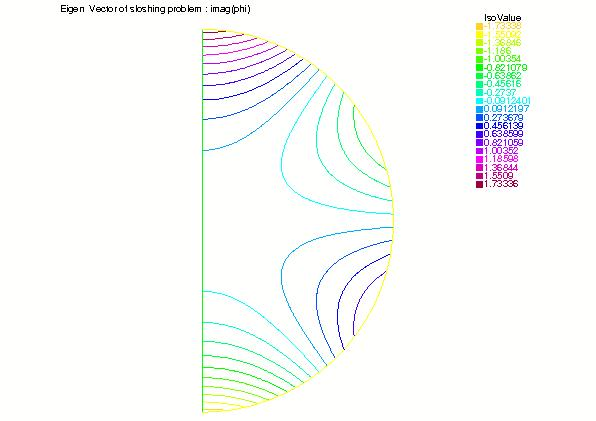
\includegraphics[width=8cm]{2_3_1_potentiel_de_vitesse.jpeg}
%\caption{potentiel de vitesse}
%\label{fig_res}
%\end{figure}

\begin{figure}[h!] 
\begin{center}
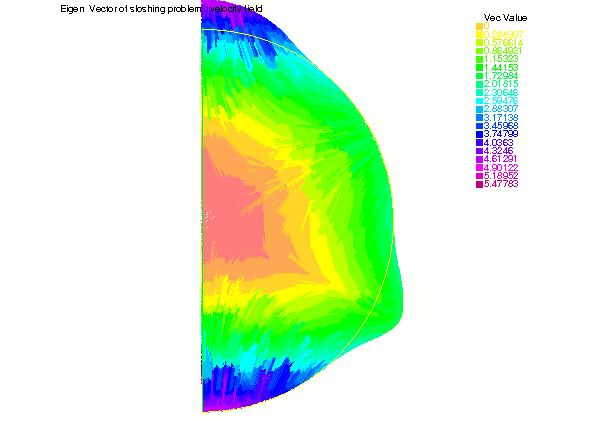
\includegraphics[width=6cm]{2_3_1_champ_de_vitesse.jpeg}
\caption{champ de vitesse}
%\label{experience}
\end{center}
\end{figure}

%\begin{figure}[!htbp]
%\centering
%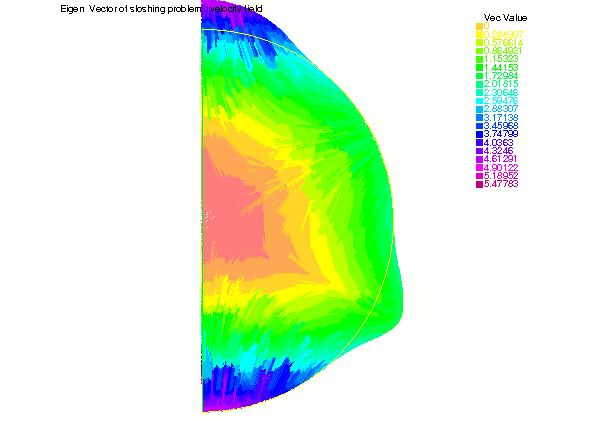
\includegraphics[width=8cm]{2_3_1_champ_de_vitesse.jpeg}
%\caption{champ de vitesse}
%\label{fig_res}
%\end{figure}

\begin{figure}[h!] 
\begin{center}
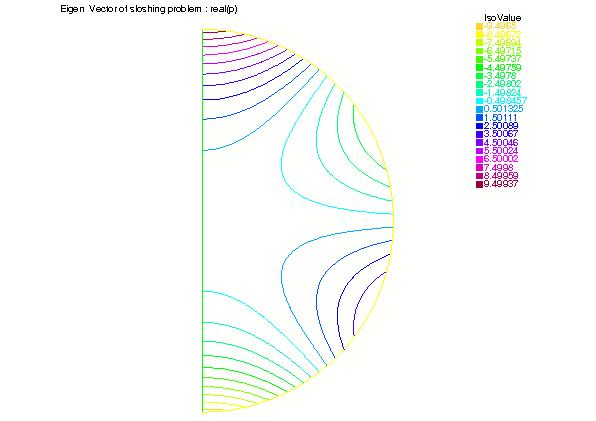
\includegraphics[width=6cm]{2_3_1_pression.jpeg}
\caption{pression}
%\label{experience}
\end{center}
\end{figure}

%\begin{figure}[!htbp]
%\centering
%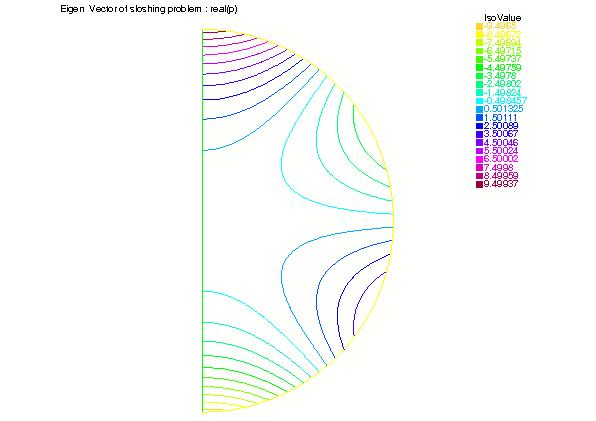
\includegraphics[width=8cm]{2_3_1_pression.jpeg}
%\caption{pression}
%\label{fig_res}
%\end{figure}

\begin{figure}[h!] 
\begin{center}
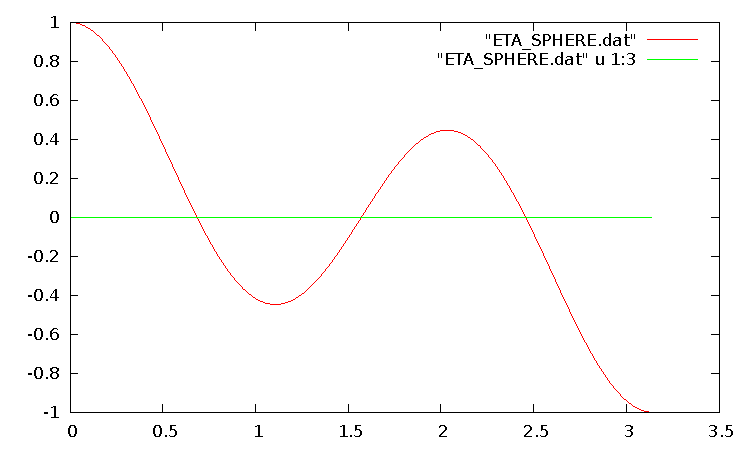
\includegraphics[width=6cm]{2_3_1_ETA_SPHERE.pdf}
\caption{déplacement de surface}
%\label{experience}
\end{center}
\end{figure}

%\begin{figure}[!htbp]
%\centering
%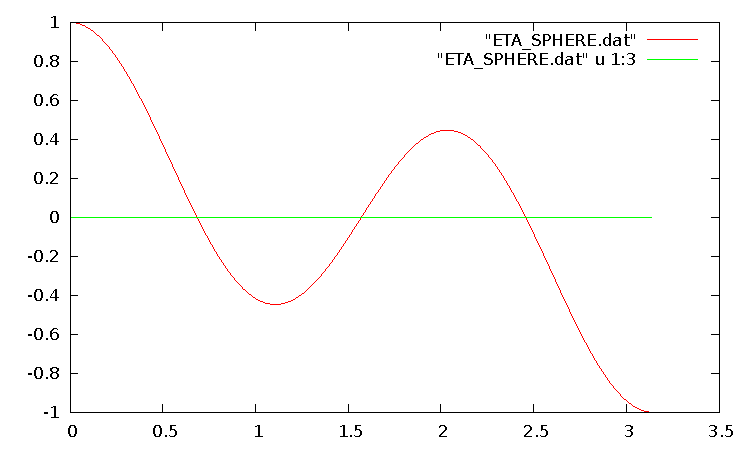
\includegraphics[width=8cm]{2_3_1_ETA_SPHERE.pdf}
%\caption{déplacement de surface}
%\label{fig_res}
%\end{figure}
%%%%%%%%%%%%%%%%%%%%%%%%%%%%%%%%%%%%%%%%%%%%%%%%%%%%
\newpage
\subsection{Cas d'une goutte avec contrainte}
Dans cette partie, on va étudier le cas d'une goutte qui oscille tout en étant tenue par un anneau circulaire. Il a mis la contrainte à la position comme la figure \ref{2_3_2_prosperetti} :






\begin{figure}[h!] 
\begin{center}
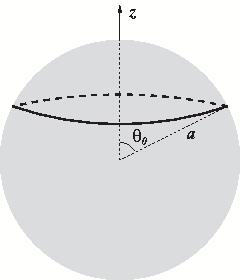
\includegraphics[width=5cm]{2_3_2_prosperetti}
\caption{Une goutte de rayon a le mouvement radial le mouvement radial duquel est prévenu par le contraint circulaire rigide}
\label{2_3_2_prosperetti}
\end{center}
\end{figure}

















%\begin{figure}[!htbp]
%\centering
%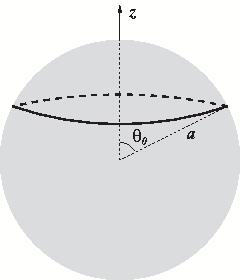
\includegraphics[width=3cm]{2_3_2_prosperetti}
%\caption{Une goutte de rayon a le mouvement radial le mouvement radial duquel est prévenu par le contraint circulaire rigide}
%\label{2_3_2_prosperetti}
%\end{figure}
%\begin{center}
%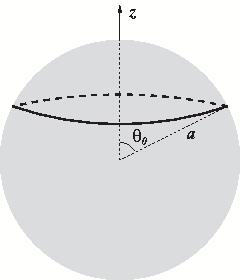
\includegraphics[width=4cm]{2_3_2_prosperetti}
%\end{center}
\newpage
Pour valider le code, on coupe le ligne surface et défini une condition limite que le déplacement de $dl$ est nul.
\begin{figure}[!htbp]
\centering
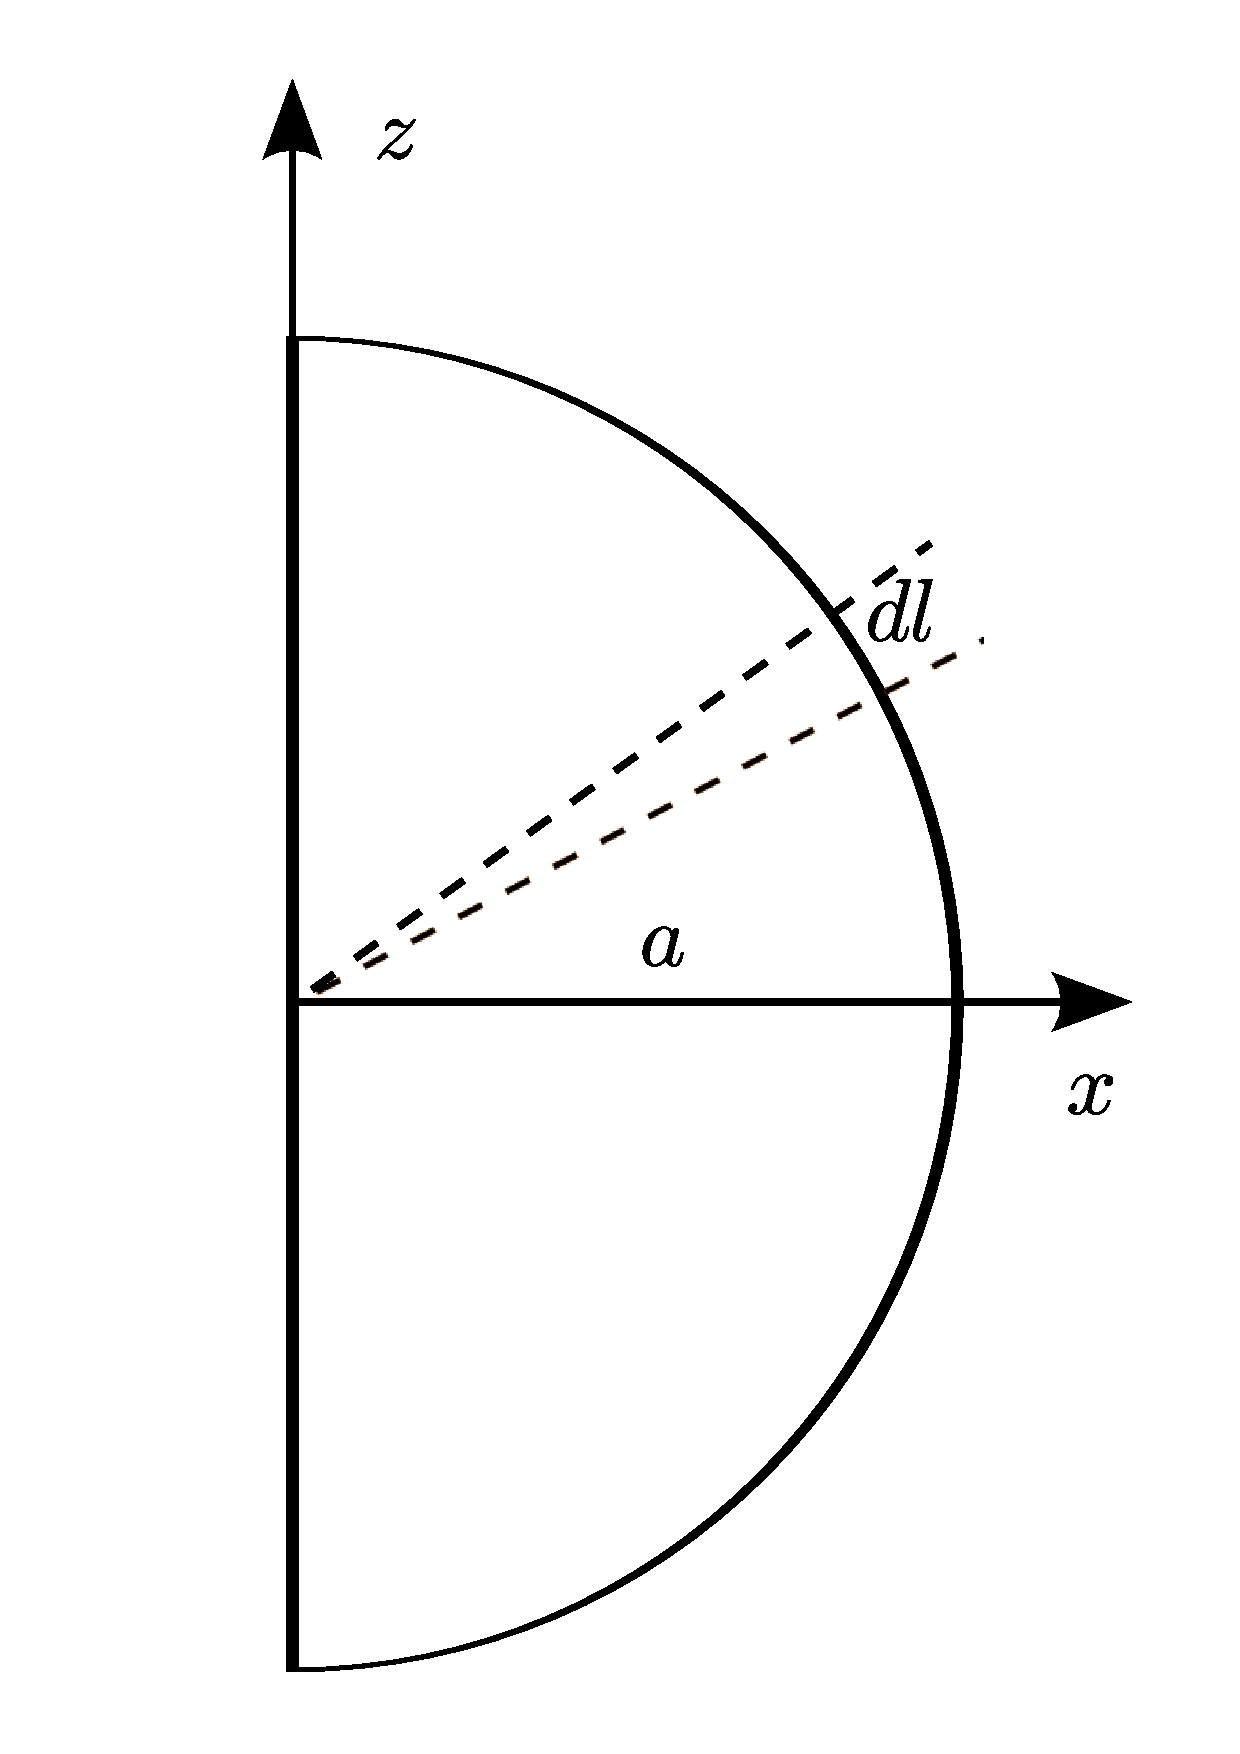
\includegraphics[width=5cm]{2_3_2_mesh}
\caption{La champ de base avec contrainte dl}
%\label{fig_res}
\end{figure}
%\begin{center}
%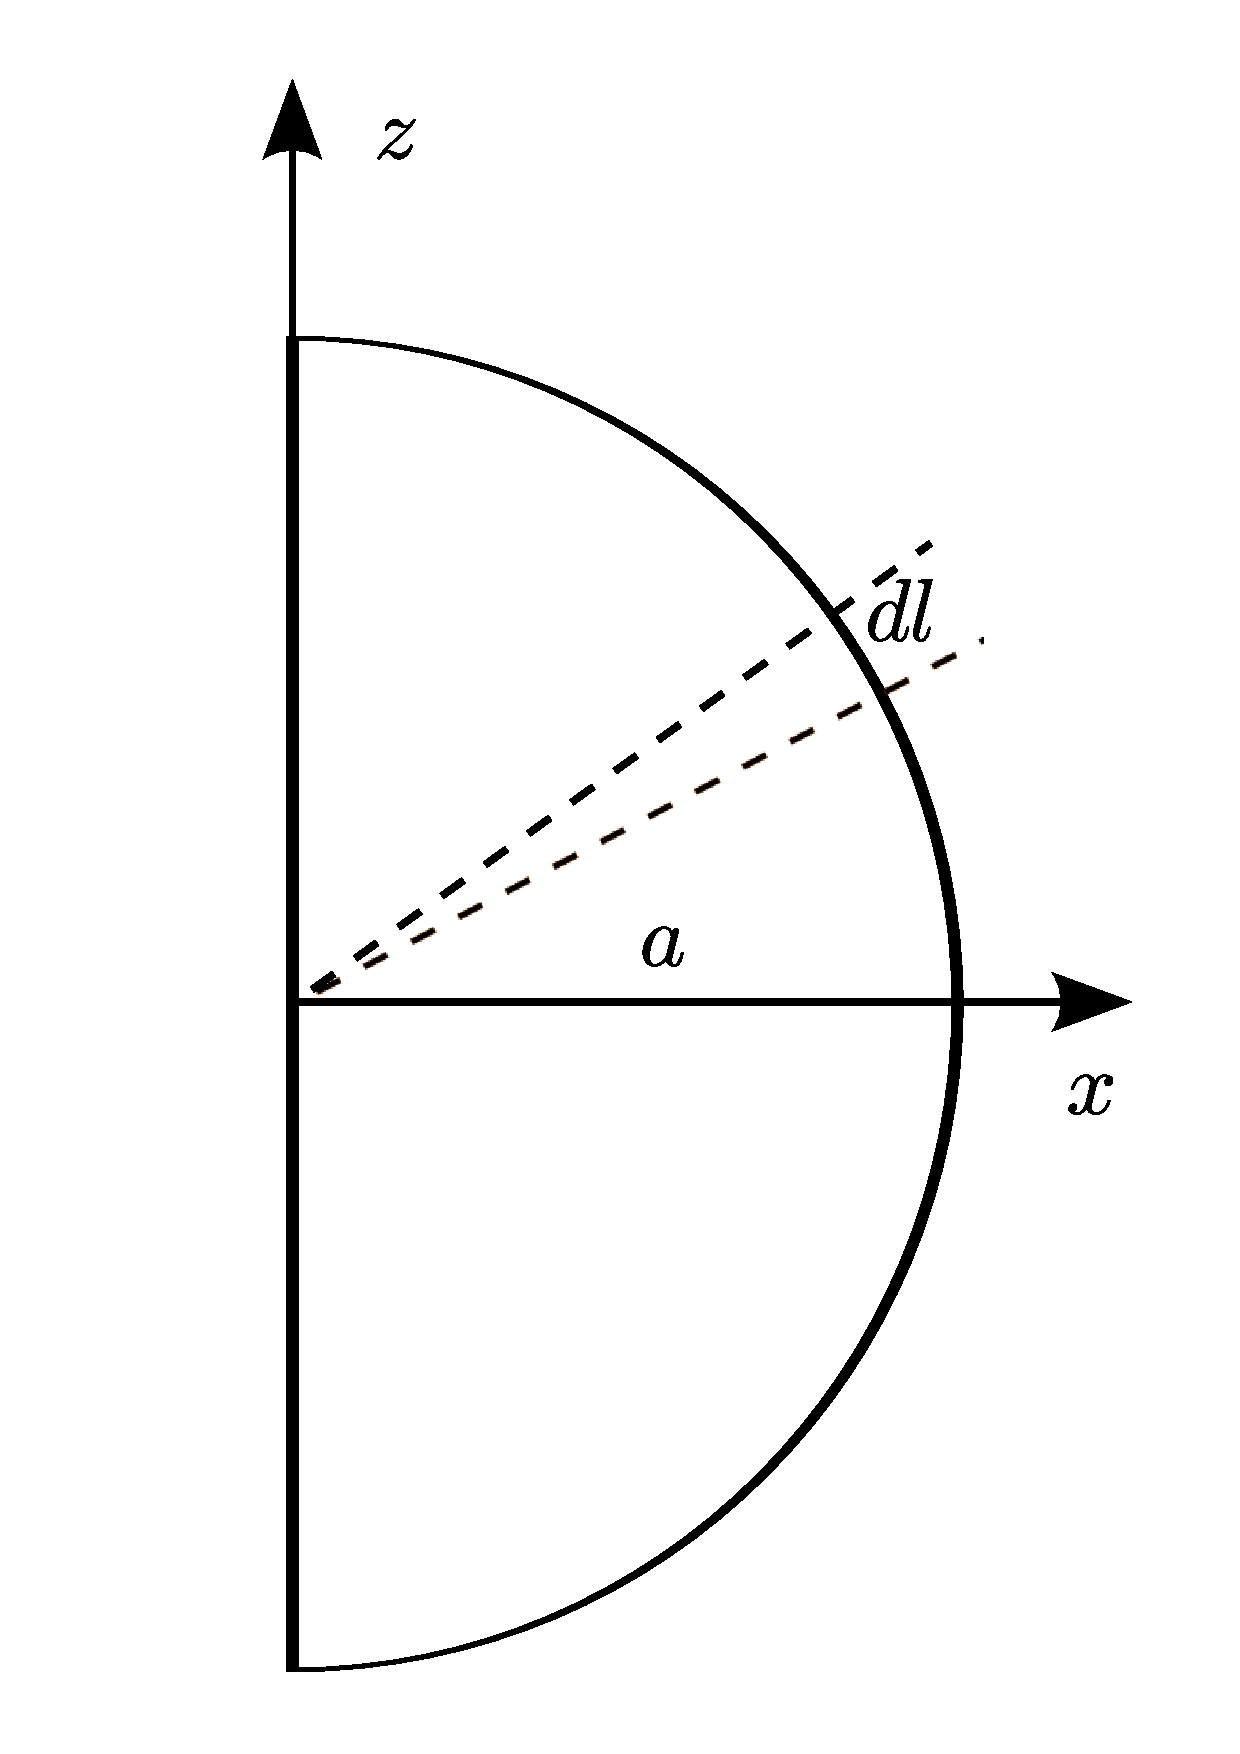
\includegraphics[width=4cm]{2_3_2_mesh}
%\end{center}
\\
Pour obtenir un point de singularité on met le noeud de $dl$ toujours égale $1$ et on espère $dl$ le plus petit possible. On va vérifier les solutions sont converges quand $dl$ tend vers 0. On choisi $N = 5505$ et $cos(\theta_0) = 0.5$.
\begin{table}[htp]
\begin{center}
    \begin{tabular}{ | l | l | l | l | l | }
    \hline
    Mode & $\omega_2$ & $\omega_3$ & $\omega_4$ \\
    \hline
    $dl = 10^{-3}$  & 2.92457 & 6.79912 & 9.95208 \\
    \hline
    $dl = 10^{-4}$  & 2.92340 & 6.79662 & 9.94586 \\
    \hline
    $dl = 10^{-5}$  & 2.92327 & 6.79633 & 9.94523 \\
    \hline
    $dl = 10^{-6}$  & 2.92326 & 6.79631 & 9.94517 \\
    \hline
    $dl = 10^{-7}$  & nul & nul & nul \\
    \hline
    Prosperetti     & 2.92733 & 6.84238 & 10.065 \\
    \hline
    \end{tabular}
\end{center}
\caption{Modes deux, trois et quatre d'une goutte avec contrainte}
\end{table}








On trouve que les solutions sont converges quand $dl$ tend vers 0, mais les solutions ne sont pas les valeurs de A. Prosperetti exactement. Peut-être on a trouvé les solutions plus précis, parce que on réalise un point de singularité. On choisi $dl = 10^{-4}$ pour le travail suivant.
\newpage
Ensuite, on fait une comparaison des fréquences obtenues avec les données de A. Prosperetti, où la fréquence $f = \frac{\omega}{2\pi}$ et $\mu_0 = cos(\theta_0)$. Ici, On choisi $N = 22839$.
\begin{table}[htp]
\begin{center}
    \begin{tabular}{ | l || l | l || l | l || l | l || }
    \hline
    Mode          &\multicolumn{2}{c||}{$\omega_2$} & \multicolumn{2}{c||}{$\omega_3$} & \multicolumn{2}{c||}{$\omega_4$} \\
    \hline
                  & Prosperetti & FreeFem++ & Prosperetti & FreeFem++ & Prosperetti & FreeFem++ \\
    \hline
    $\mu_0 = 0$    & 0.7138      & 0.7028    & 0.8717      & 0.8718    & 1.706       & 1.682 \\
    \hline
    $\mu_0 = 0.2$  & 0.6197      & 0.6142    & 1.020       & 1.011     & 1.474       & 1.465 \\
    \hline
    $\mu_0 = 0.5$  & 0.4659      & 0.4651    & 1.089       & 1.081     & 1.602       & 1.581 \\
    \hline
    $\mu_0 = 0.7$  & 0.5287      & 0.5234    & 0.9116      & 0.9095    & 1.555       & 1.546 \\
    \hline
    $\mu_0 = 0.9$  & 0.6728      & 0.6671    & 1.177       & 1.159     & 1.492       & 1.469 \\
    \hline
    \end{tabular}
\end{center}
\caption{Comparaison des modes deux, trois et quatre d'une goutte avec contrainte}
\end{table}


\begin{figure}[!htbp]
\centering
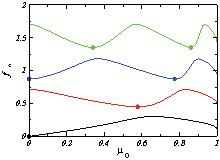
\includegraphics[width=10cm]{2_3_2_contrainte_Prosperetti.jpeg}
\caption{Les lignes des modes pour une goutte avec contrainte obtenus par Prosperetti}
%\label{fig_res}
\end{figure}
\begin{figure}[!htbp]
\centering
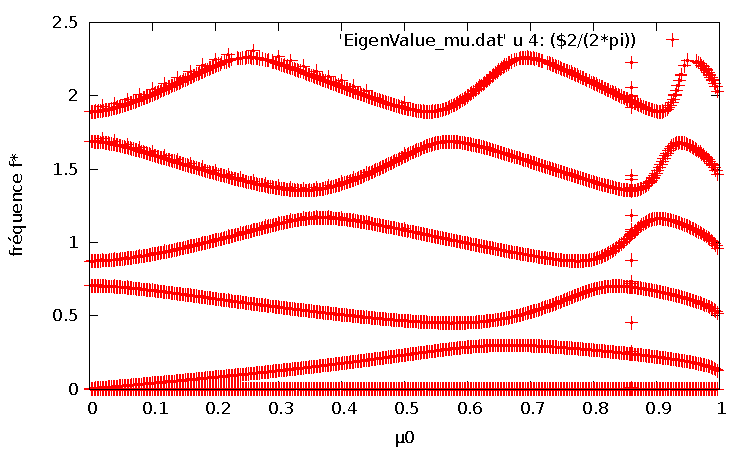
\includegraphics[width=10cm]{2_3_2_contrainte_FreeFem}
\caption{Les lignes des modes pour une goutte avec contrainte obtenus obtenus parFreeFem++, $N \approx 1400$}
%\label{fig_res}
\end{figure}













\newpage
Enfin, par exemple $N = 8643$ et $\mu_0 = 0.5$, on choisi le troisième mode $\omega_3 = 6.7966$ et visualise le potentiel de vitesse, le champ de vitesse, la pression et le déplacement de surface. En même temps, on fait une comparaison des résultats avec le cas sans contrainte.
\begin{figure}
\begin{minipage}[h!]{0.5\linewidth}
\centering
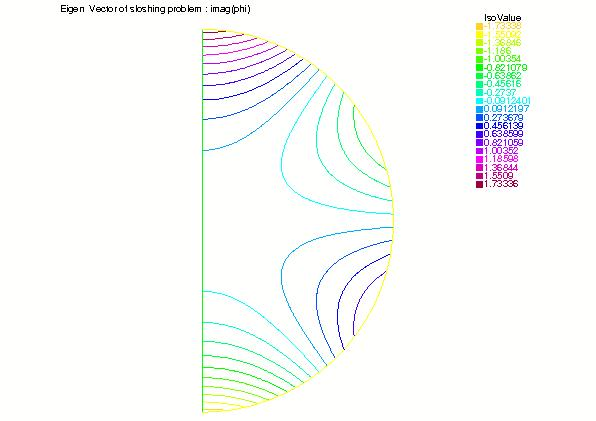
\includegraphics[width=8cm]{2_3_1_potentiel_de_vitesse.jpeg}
\caption{potentiel de vitesse sans contrainte }
%\label{fig:side:a}
\end{minipage}
\begin{minipage}[h!]{0.5\linewidth}
\centering
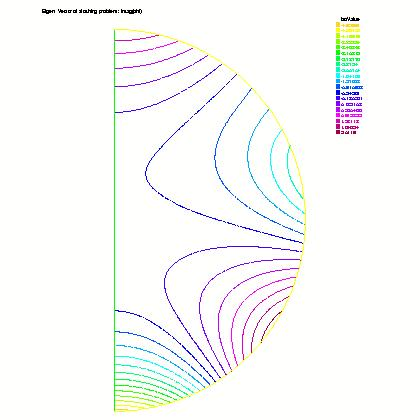
\includegraphics[width=6cm]{2_3_2_potentiel_de_vitesse.jpeg}
\caption{potentiel de vitesse avec contrainte}
%\label{fig:side:b}
\end{minipage}
\end{figure}


\begin{figure}
\begin{minipage}[h!]{0.5\linewidth}
\centering
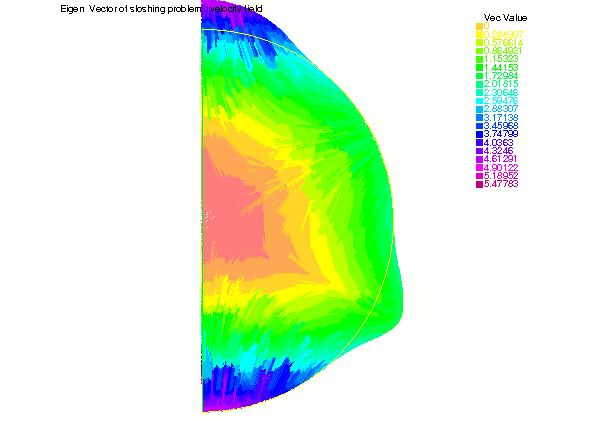
\includegraphics[width=8cm]{2_3_1_champ_de_vitesse.jpeg}
\caption{champ de vitesse sans contrainte }
%\label{fig:side:a}
\end{minipage}
\begin{minipage}[h!]{0.5\linewidth}
\centering
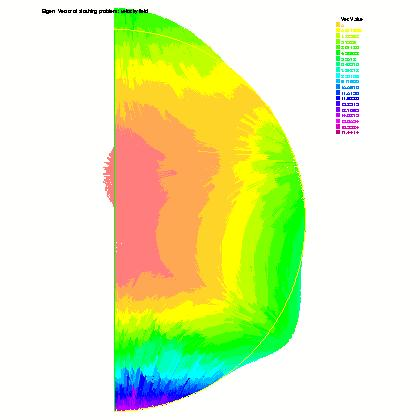
\includegraphics[width=6cm]{2_3_2_champ_de_vitesse.jpeg}
\caption{champ de vitesse avec contrainte}
%\label{fig:side:b}
\end{minipage}
\end{figure}
\begin{figure}
\begin{minipage}[h!]{0.5\linewidth}
\centering
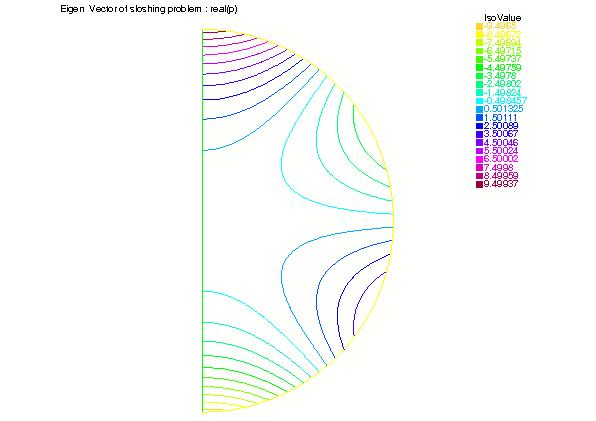
\includegraphics[width=8cm]{2_3_1_pression.jpeg}
\caption{pression sans contrainte }
%\label{fig:side:a}
\end{minipage}
\begin{minipage}[h!]{0.5\linewidth}
\centering
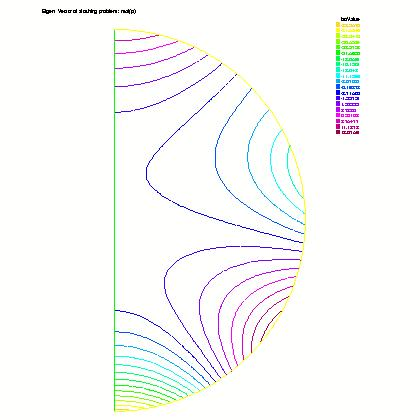
\includegraphics[width=6cm]{2_3_2_pression.jpeg}
\caption{pression avec contrainte}
%\label{fig:side:b}
\end{minipage}
\end{figure}
\begin{figure}
\begin{minipage}[h!]{0.5\linewidth}
\centering
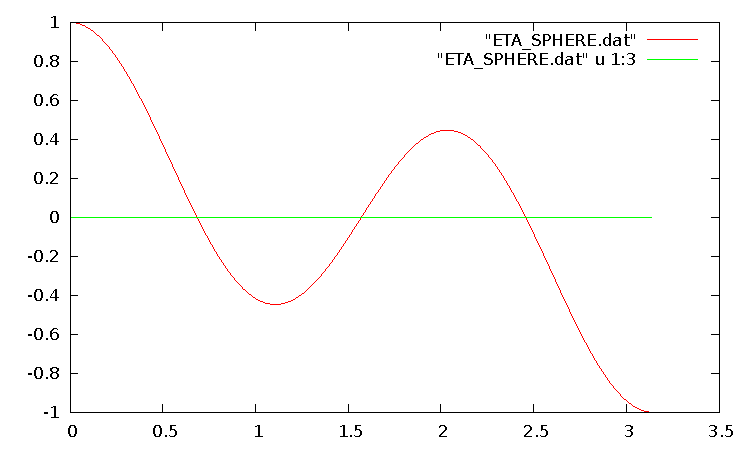
\includegraphics[width=6cm]{2_3_1_ETA_SPHERE.pdf}
\caption{déplacement de surface sans contrainte }
%\label{fig:side:a}
\end{minipage}
\begin{minipage}[h!]{0.5\linewidth}
\centering
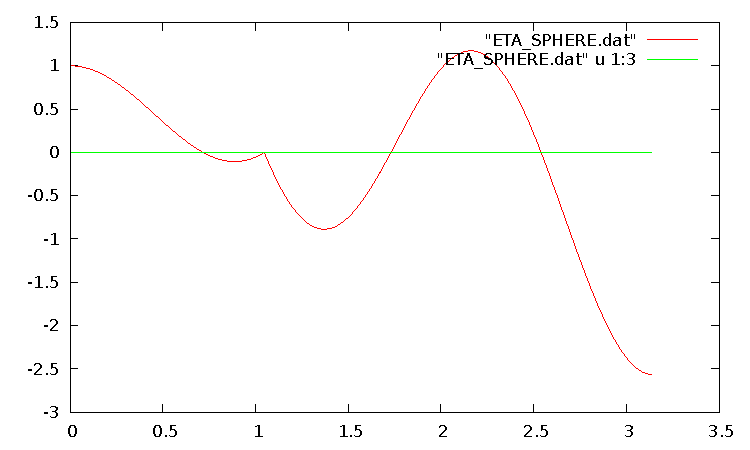
\includegraphics[width=6cm]{2_3_2_ETA_SPHERE.pdf}
\caption{déplacement de surface avec contrainte}
%\label{fig:side:b}
\end{minipage}
\end{figure}












%%%%%%%%%%%%%%%%%%%%%%%%%%%%%%%%%%%%%%%%%%%%%%%%%%%%
\newpage
\subsection{Cas d'une bulle sans contrainte}
Pour le cas d'une bulle, on modifie l'espace d'élément fini seulement comme au-dessous :


\begin{figure}[h!] 
\begin{center}
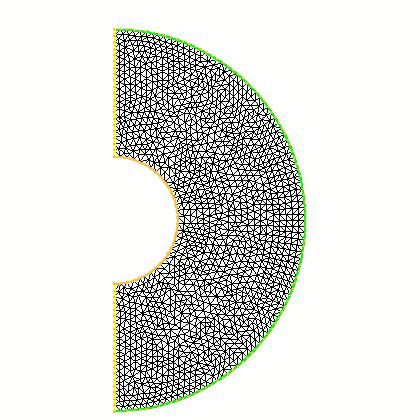
\includegraphics[width=6cm]{2_3_3_Bulle}
\caption{La champ de base pour une bulle}
%\label{2_3_2_prosperetti}
\end{center}
\end{figure}


%\begin{center}
%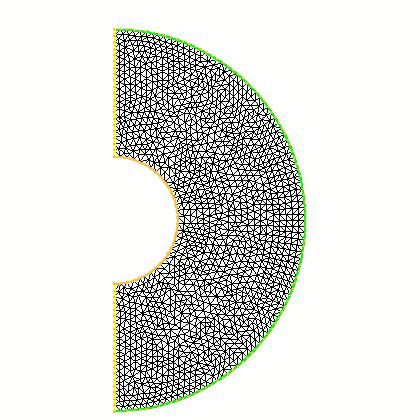
\includegraphics[width=8cm]{2_3_3_Bulle}
%\end{center}
On sait que la valeur propre d'une bulle non visqueux est généralisé par H. Lamb sous la forme suivante :
\begin{eqnarray*}
{\omega_n}^2 = (n-1) (n+1) (n+2) \frac{\sigma}{\rho a^3}
\end{eqnarray*}
On met $\sigma = 1$, $\rho = 1$, $a = 1$, le rayon de grand demi circle $R_{MAX} = 5$ et le parametre de pénalisation $\epsilon = 10^{-7}$ pour comparer les données dans le tableau suivant :


\begin{table}[htp]
\begin{center}
    \begin{tabular}{ | l | l | l | l | l | }
    \hline
    Mode & $\omega_2$ & $\omega_3$ & $\omega_4$ \\
    \hline
    $N = 388  $ & 3.4904 & 6.41201 & 9.68805 \\ %10
    \hline
    $N = 1539 $ & 3.4695 & 6.34761 & 9.53215 \\ %20
    \hline
    $N = 3676 $ & 3.4660 & 6.33364 & 9.50818 \\ %30
    \hline
    $N = 6293 $ & 3.4646 & 6.32973 & 9.49995 \\ %40
    \hline
    $N = 10110$ & 3.4638 & 6.32786 & 9.49457 \\ %50
    \hline
    $N = 14567$ & 3.4635 & 6.32693 & 9.49236 \\ %60
    \hline
    $N = 19709$ & 3.4633 & 6.32619 & 9.49102 \\ %70
    \hline
    $N = 25637$ & 3.4631 & 6.32586 & 9.48988 \\ %80
    \hline
    $N = 32479$ & 3.4630 & 6.32553 & 9.48934 \\ %90
    \hline
    $N = 40057$ & 3.4629 & 6.32533 & 9.48875 \\ %100
    \hline
    Théorique   & 3.4641 & 6.32456 & 9.48683 \\
    \hline
    \end{tabular}
\end{center}
\caption{Modes deux, trois et quatre d'une goutte libre}
\end{table}
%\newline
Avec $N$ le nombre de triangles constituant le maillage.
\\[0.25cm]
Remarque : On choisi $R_{MAX} = 5$ pour la raison de simplifier le calcul et étudier qualitativement seulement.
%%%%%%%%%%%%%%%%%%%%%%%%%%%%%%%%%%%%%%%%%%%%%%%%%%%%
\newpage
\subsection{Cas d'une bulle avec contrainte}
Dans ce cas, on fait une comparaison qualitativement des fréquences obtenues par FreeFem++ avec les données de A. Prosperetti seulement.
\begin{figure}[!htbp]
\centering
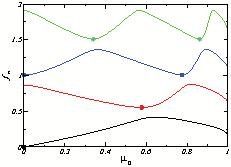
\includegraphics[width=10cm]{2_3_4_contrainte_Prosperetti.jpeg}
\caption{Les lignes des modes pour une goutte avec contrainte obtenus par Prosperetti}
%\label{fig_res}
\end{figure}
\begin{figure}[!htbp]
\centering
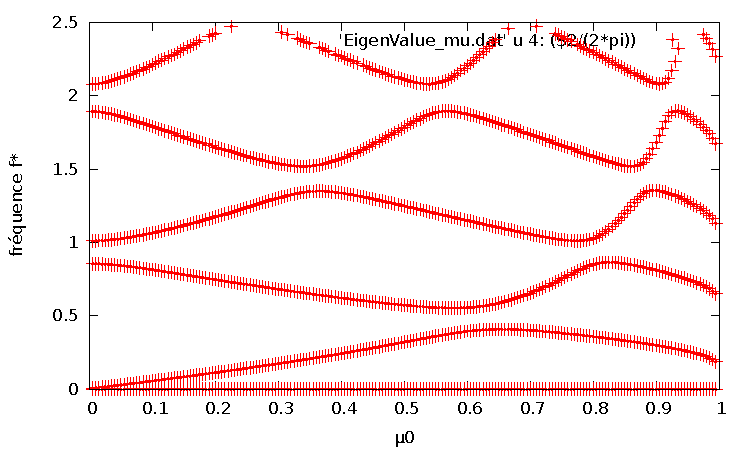
\includegraphics[width=10cm]{2_3_4_contrainte_FreeFem}
\caption{Les lignes des modes pour une goutte avec contrainte obtenus par Prosperetti}
%\label{fig_res}
\end{figure}



%%%%%%%%%%%%%%%%%%%%%%%%%%%%%%%%%%%%%%%%%%%%%%%%%%%%%%%%%%%%%%%%%%%%%%%%%%%%%%%%%%%%%%%%%%%%%%%%%%%%%%%%%
%%%%%%%%%%%%%%%%%%%%%%%%%%%%%%%%%%%%%%%%%%%%%%%%%%%%%%%%%%%%%%%%%%%%%%%%%%%%%%%%%%%%%%%%%%%%%%%%%%%%%%%%%
%%%%%%%%%%%%%%%%%%%%%%%%%%%%%%%%%%%%%%%%%%%%%%%%%%%%%%%%%%%%%%%%%%%%%%%%%%%%%%%%%%%%%%%%%%%%%%%%%%%%%%%%%
\chapter{Une gouttelette de liquide immergée dans un autre fluide non visqueux}
Dans ce chapitre, on va vérifier la formule au-dessous :
\begin{eqnarray}
{\omega_n}^2 = \frac{ (n-1) n (n+1) (n+2) \sigma }{ ( \rho_1 (n+1) + \rho_2 n ) a^3 }
\end{eqnarray}
Dans le cadre de ce rapport, on défini $\rho_1$ est la masse volumique de la gouttelette de liquide (Fluide 1) et $\rho_2$ est la masse volumique du fluide où la gouttelette de liquide immergée (Fluide 2).
%%%%%%%%%%%%%%%%%%%%%%%%%%%%%%%%%%%%%%%%%%%%%%%%%%%%%%%%%%%%%%%%%%%%%%%%%%%%%%%%%%%%%%%%%%%%%%%%%%%%%%%%%
\section{Position du problème}
%%%%%%%%%%%%%%%%%%%%%%%%%%%%%%%%%%%%%%%%%%%%%%%%%%%%
\subsection{Étude du champ de base}
%\begin{center}
%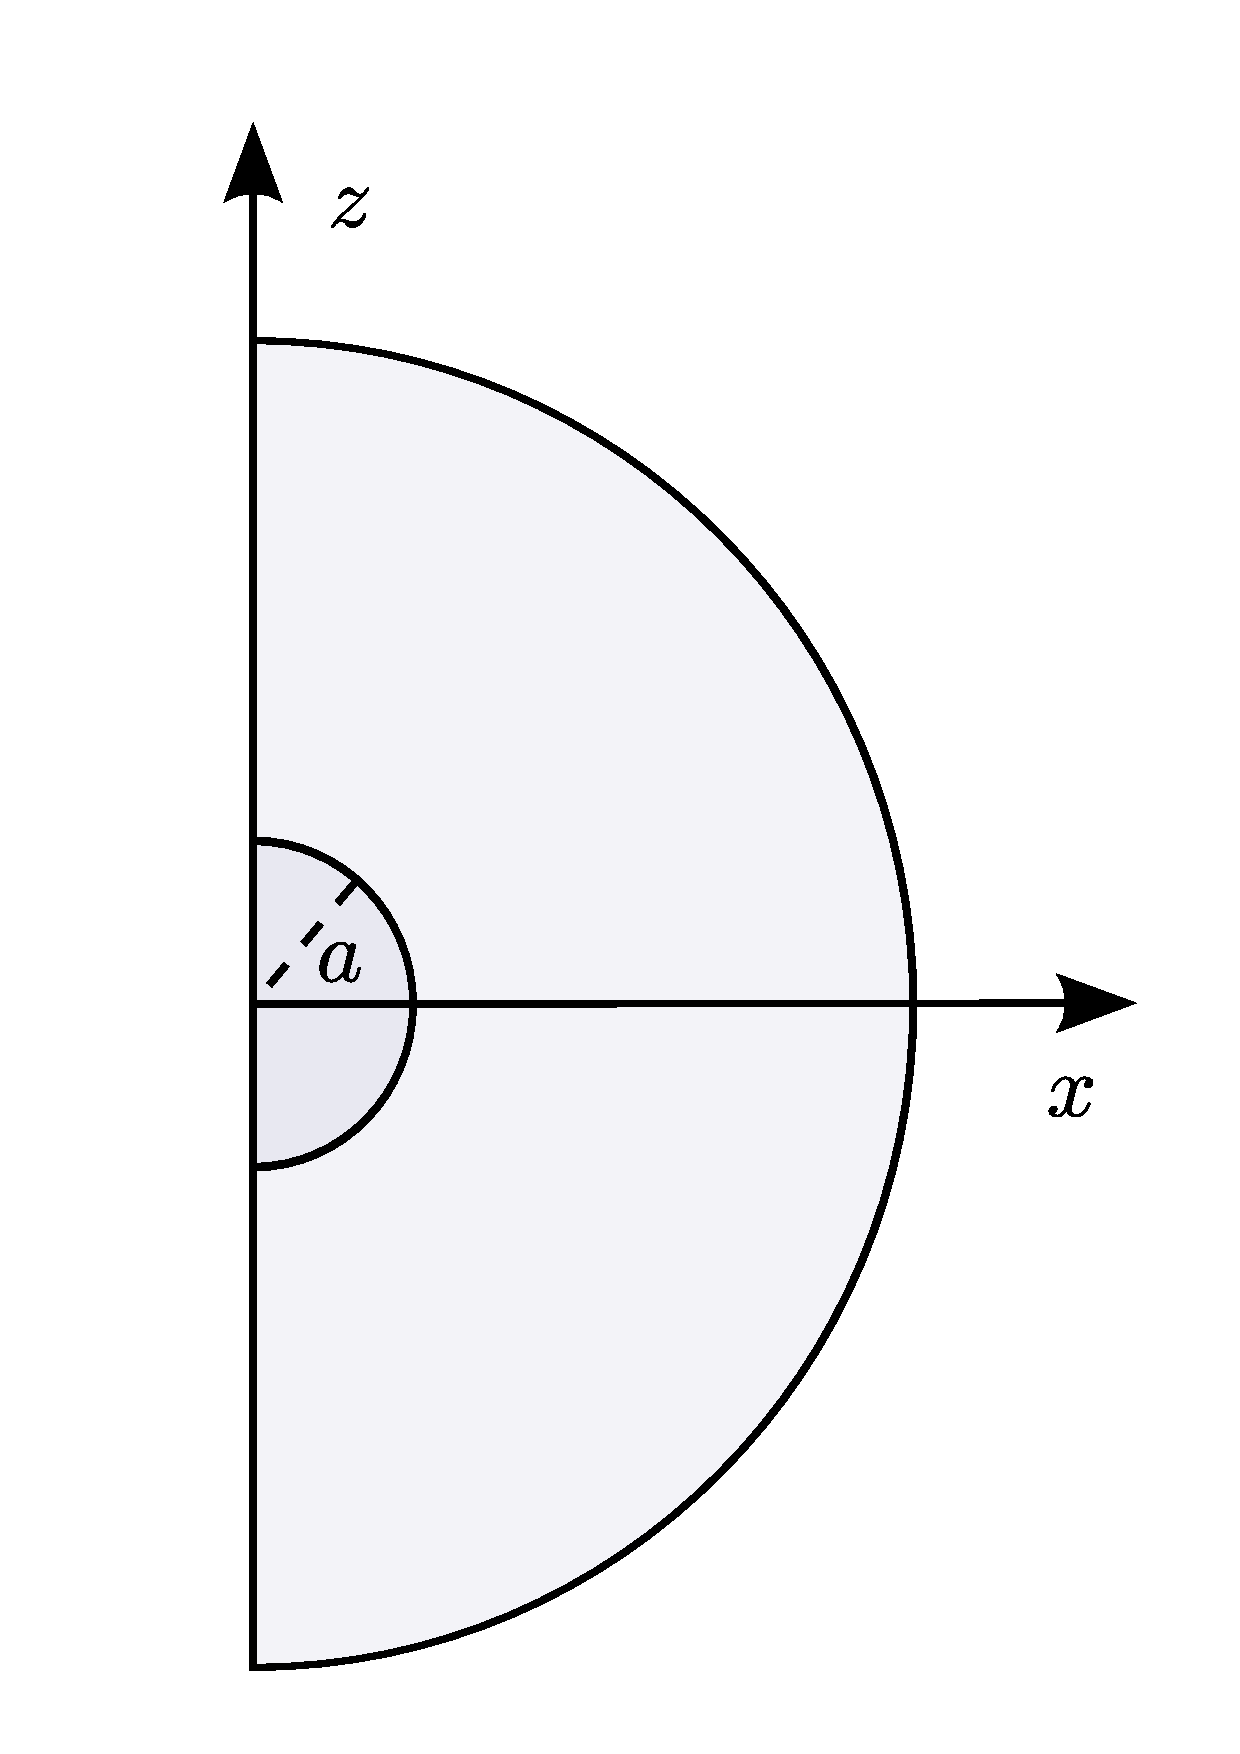
\includegraphics[width=4cm]{3_1_1}
%\end{center}
\begin{figure}[!htbp]
\centering
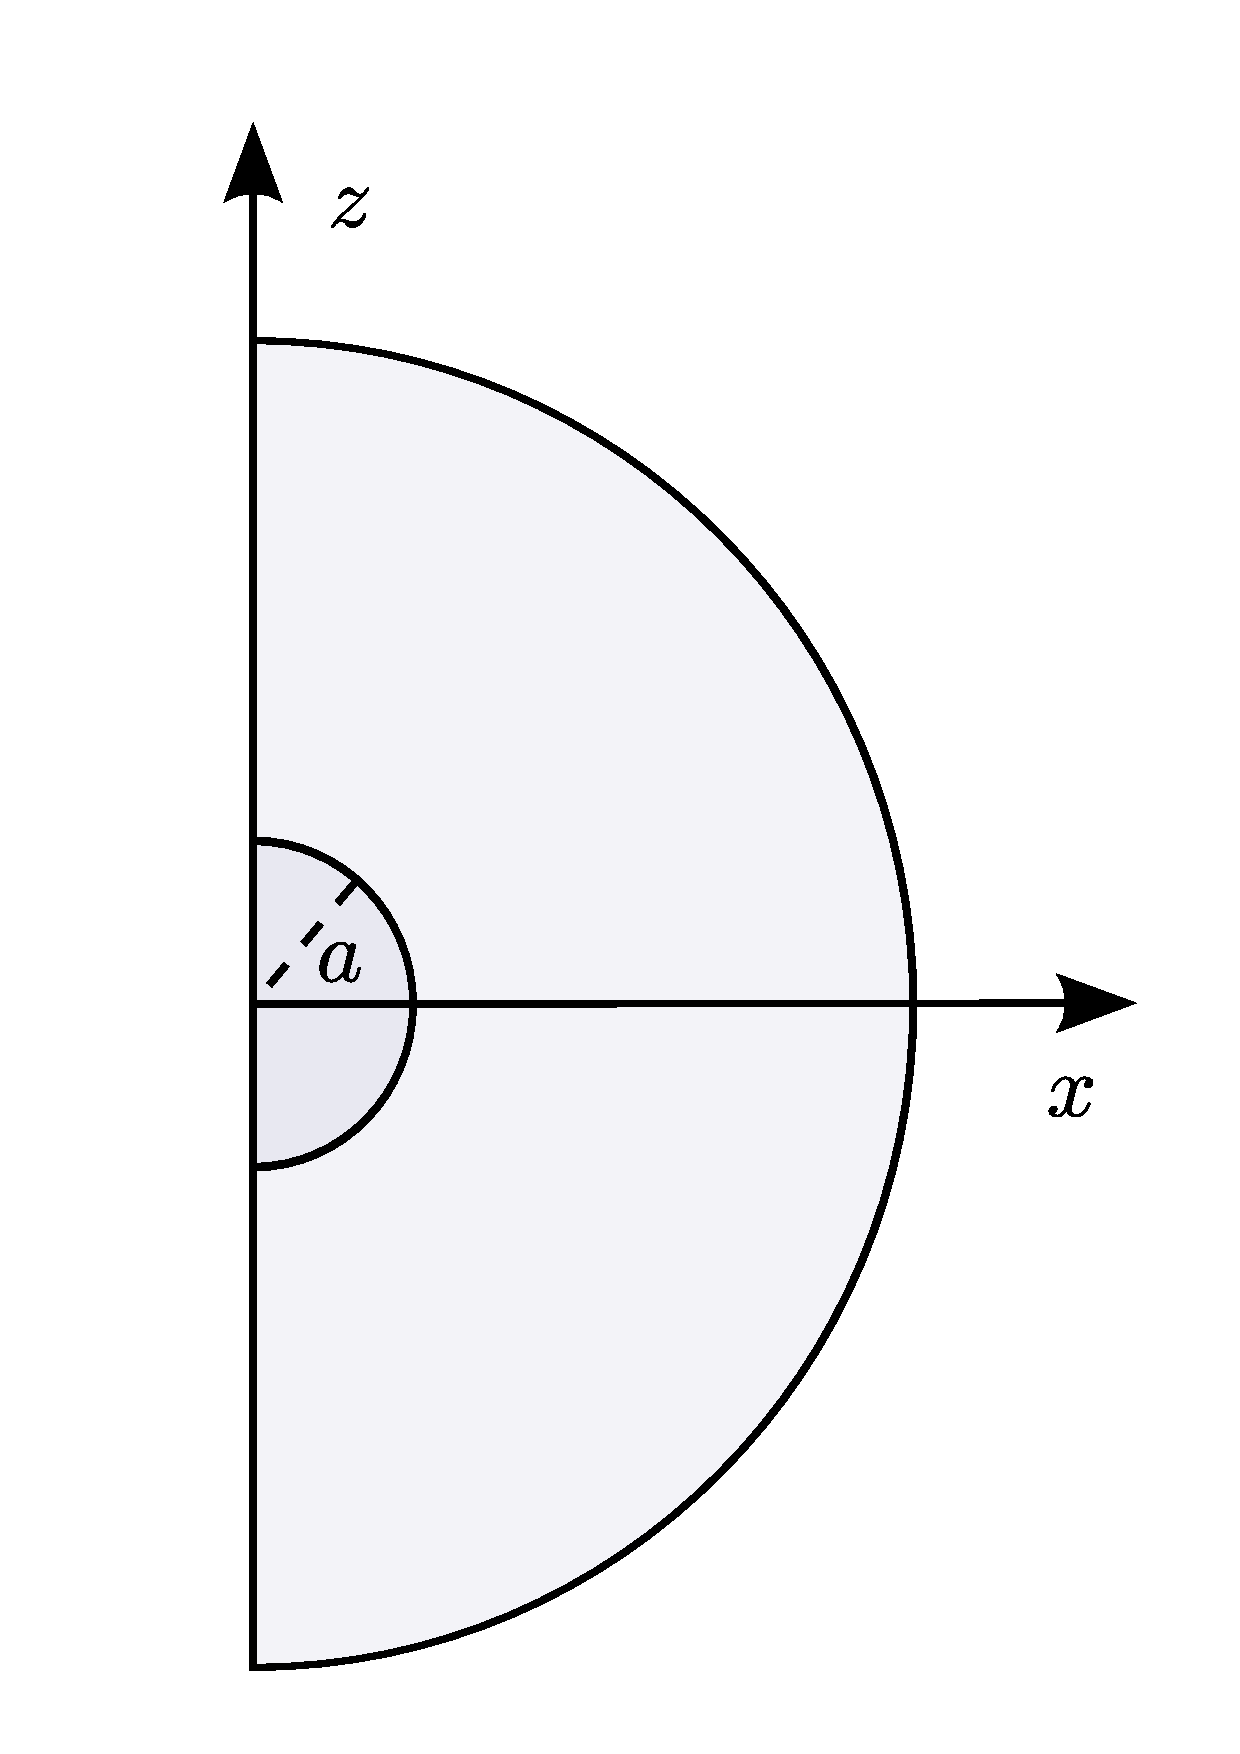
\includegraphics[width=3cm]{3_1_1}
\caption{La champ de base pour deux fluides}
%\label{fig_res}
\end{figure}
Nous adopterons le système de coordonnées sphériques $(r,\theta,\phi)$ centré au centre de la goutte.
\begin{tabbing}
Notons :\\
$a$\,\    \= : le rayon d'équilibre de la goutte\\
$\varPhi_1$ \> : le potentiel de vitesse du fluide 1\\
$\varPhi_2$ \> : le potentiel de vitesse du fluide 2\\
$P_1$       \> : la pression du côté intérieur du fluide 1\\
$P_2$       \> : la pression du côté intérieur du fluide 2\\
$H$       \> : le rayon de la goutte
\end{tabbing}
%%%%%%%%%%%%%%%%%%%%%%%%%%%%%%%%%%%%%%%%%%%%%%%%%%%%
\subsection{Équations générales}
\begin{eqnarray}\label{pb:31}         %方程组开始
\left\{                              %方程组的左边包括大括号\{
\begin{array}{lll}                   %设定列阵的格式:{lll}是三个L,表示三列的对齐方式为Left对齐
\Delta \varPhi_1 = 0                                                                                     & \text{dans le volume $\Omega_1$}    \\%&——分隔列的标记,\\——表示换行
\Delta \varPhi_2 = 0                                                                                     & \text{dans le volume $\Omega_2$}    \\%&——分隔列的标记,\\——表示换行
P_1 + \rho_1\ \frac{\partial}{\partial t}\varPhi_1 = 0                                                   & \text{dans le volume $\Omega_1$}    \\%&同上
P_2 + \rho_2\ \frac{\partial}{\partial t}\varPhi_2 = 0                                                   & \text{dans le volume $\Omega_2$}    \\%&同上
\frac{\partial}{\partial t} H = \nabla \varPhi_1 \cdot \vec{n} = \frac{\partial}{\partial r} \varPhi_1   & \text{sur la surface libre $S$ (Condition cinématique)}      \\
\frac{\partial}{\partial t} H = - \nabla \varPhi_2 \cdot \vec{n} = - \frac{\partial}{\partial r} \varPhi_2   & \text{sur la surface libre $S$ (Condition cinématique)}      \\
P_2 - P_1 = \sigma\ \mathscr{C}                              & \text{sur la surface libre $S$ (Condition dynamique)}   % \mathcal{C} ou \mathscr{C}
\end{array}                          %方程列阵的结束
\right.                              %方程组的右边无符号,利用“.“来标示
\end{eqnarray}                       %方程组结束
\begin{flalign*}
\text{où}   & &\\
\sigma      &: \text{le coefficient de tension superficielle} &\\
\mathscr{C} &: \text{la courbure moyenne de l'interface} &
\end{flalign*}
%%%%%%%%%%%%%%%%%%%%%%%%%%%%%%%%%%%%%%%%%%%%%%%%%%%%
\subsection{Décomposition modale}
On considère maintenant l'oscillation linéaire d'une goutte sphérique par rapport à la position d'équilibre :
\begin{eqnarray*}
\varPhi_1   &=& \varPhi_{10} + \varphi_1(r,\theta,\phi)\ e^{- i \omega t} \\
\varPhi_2   &=& \varPhi_{20} + \varphi_2(r,\theta,\phi)\ e^{- i \omega t} \\
P_1         &=& P_{10} + p_1(r,\theta,\phi)\ e^{- i \omega t}\\
P_2         &=& P_{20} + p_2(r,\theta,\phi)\ e^{- i \omega t}\\
H           &=& a + \varepsilon\ \eta(\theta,\phi)\ e^{- i \omega t}
\end{eqnarray*}
Pour la courbe, on a
\begin{eqnarray*}
\mathscr{C} = \mathscr{C}_0 + \varepsilon \ \mathscr{C}_1 + o(\varepsilon^2)
\end{eqnarray*}
où
\begin{eqnarray*}
\mathscr{C}_1 = - \left[\ \frac{2}{a^2} \ \eta
                          + \frac{1}{a^2 \sin\theta} \frac{\partial}{\partial \theta}(\ \sin\theta \ \frac{\partial}{\partial \theta} \eta \ )\ \right]\ e^{- i \omega t}.
\end{eqnarray*}
%%%%%%%%%%%%%%%%%%%%%%%%%%%%%%%%%%%%%%%%%%%%%%%%%%%%
\subsection{Linéarisation des équations}
La linéarisation des équations s'effectue en remplaçant dans le système d'équations d'équilibre \eqref{pb:31} le potentiel de vitesse, le champ de pression et la courbure par leur décomposition, puis en conservant uniquement les termes d'ordre 1 par rapport aux petites perturbation introduites. Nous obtenons ainsi le problème linéaire suivant :
\begin{eqnarray}\label{pb:32}         %方程组开始
\left\{                              %方程组的左边包括大括号\{
\begin{array}{lll}                   %设定列阵的格式:{lll}是三个L,表示三列的对齐方式为Left对齐
\Delta \varphi_1 = 0                                                                                     & \text{dans le volume $\Omega_1$}    \\%&——分隔列的标记,\\——表示换行
\Delta \varphi_2 = 0                                                                                     & \text{dans le volume $\Omega_2$}    \\%&——分隔列的标记,\\——表示换行
p_1 + \lambda\ \rho_1\ \varphi_1 = 0                                                        & \text{dans le volume $\Omega_1$}    \\%&同上
p_2 + \lambda\ \rho_2\ \varphi_2 = 0                                                        & \text{dans le volume $\Omega_2$}    \\%&同上
\lambda\ \eta = \nabla \varphi_1 \cdot \vec{n} = \frac{\partial}{\partial r} \varphi_1      & \text{sur la surface libre $S$ (Condition cinématique)}      \\
\lambda\ \eta = - \nabla \varphi_2 \cdot \vec{n} = - \frac{\partial}{\partial r} \varphi_2      & \text{sur la surface libre $S$ (Condition cinématique)}      \\
p_2 -p_1 = - \sigma\ \left[\ \frac{2}{a^2} \ \eta
                      + \frac{1}{a^2 \sin\theta} \frac{\partial}{\partial \theta}(\ \sin\theta \ \frac{\partial}{\partial \theta} \eta \ )\ \right]
& \text{sur la surface libre $S$ (Condition dynamique)}   % \mathcal{C} ou \mathscr{C}
\end{array}                          %方程列阵的结束
\right.                              %方程组的右边无符号,利用“.“来标示
\end{eqnarray}                       %方程组结束
Avec $\lambda = - i \omega t$ les valeurs propre recherchés.
%%%%%%%%%%%%%%%%%%%%%%%%%%%%%%%%%%%%%%%%%%%%%%%%%%%%%%%%%%%%%%%%%%%%%%%%%%%%%%%%%%%%%%%%%%%%%%%%%%%%%%%%%
\section{Modélisation numérique}
%%%%%%%%%%%%%%%%%%%%%%%%%%%%%%%%%%%%%%%%%%%%%%%%%%%%
\subsection{Formulation variationnelle}
Pour l'implémentation de ces équations sous FreeFem++ il convient de mettre en place une formulation variationnelle (ou formulation faible). Pour cela, introduit des fonction test $\varphi^*_1, \varphi^*_2, p^*_1, p^*_2, \eta^*$ associées à $\varphi_1, \varphi_2, p_1, p_2, \eta$, où $(\varphi^*_1, p^*_1)$ définis sur $\Omega_1$, $(\varphi^*_2, p^*_2)$ définis sur $\Omega_2$, $\eta^*$ défini sur $S$.
\\[0.25cm]
La formulation variationnelle du problème \eqref{pb:32} se met alors en plusieurs étapes. Dans un premiers temps, on multiplie scalairement les équation du problème \eqref{pb:32} par leur fonction test associée :
\\[0.25cm]
$\forall \varphi^*_1, \varphi^*_2, p^*_1, p^*_2, \eta^*$
\begin{eqnarray*}
\left\{
\begin{array}{rcl}
\left(\ \Delta \varphi_1\ \right) \cdot \varphi^*_1 &=& 0 \\
\left(\ \Delta \varphi_2\ \right) \cdot \varphi^*_2 &=& 0 \\
\left(\ p_1 + \lambda\ \rho_1\ \varphi_1\ \right) \cdot p^*_1 &=& 0 \\
\left(\ p_2 + \lambda\ \rho_2\ \varphi_2\ \right) \cdot p^*_2 &=& 0 \\
\left(\ p_2 - p_1 + \sigma\ \left[\ \frac{2}{a^2} \ \eta
                    + \frac{1}{a^2 \sin\theta} \frac{\partial}{\partial \theta}(\ \sin\theta \ \frac{\partial}{\partial \theta} \eta \ )\ \right]\ \right) \cdot \eta^* &=& 0
\end{array}
\right.
\end{eqnarray*}
Ensuite, on intègres ces trois équations. On obtient alors :
\\[0.25cm]
$\forall \varphi^*_1, \varphi^*_2, p^*_1, p^*_2, \eta^*$
\begin{eqnarray*}
\left\{
\begin{array}{rcl}
(\ \Delta \varphi_1 ,\ \varphi^*_1 \ )_{\Omega_1} &=& 0 \\
(\ \Delta \varphi_2 ,\ \varphi^*_2 \ )_{\Omega_2} &=& 0 \\
(\ - p_1 ,\ p^*_1 \ )_{\Omega_1} &=& \lambda\ (\ \rho_1\ \varphi_1 ,\ p^*_1 \ )_{\Omega_1} \\
(\ - p_2 ,\ p^*_2 \ )_{\Omega_2} &=& \lambda\ (\ \rho_2\ \varphi_2 ,\ p^*_2 \ )_{\Omega_2} \\
<\ p_2 - p_1 + \sigma\ \left[\ \frac{2}{a^2} \ \eta
                       + \frac{1}{a^2 \sin\theta} \frac{\partial}{\partial \theta}(\ \sin\theta \ \frac{\partial}{\partial \theta} \eta \ )\ \right] ,\ \eta^* \ >_S &=& 0
\end{array}
\right.
\end{eqnarray*}
Enfin, la condition cinématique est introduite au sein de cette formulation grâce à la formule de Green s'écrit :
\\[0.25cm]
$\forall \varphi^*_1$,
\begin{eqnarray*}
(\ \Delta \varphi_1 ,\ \varphi^*_1 \ )_{\Omega_1} = - (\ \nabla \varphi_1 ,\ \nabla \varphi^*_1 \ )_{\Omega_1} + <\ \nabla \varphi_1 \cdot \vec{n},\ \varphi^*_1 \ >_S
\end{eqnarray*}
$\forall \varphi^*_2$,
\begin{eqnarray*}
(\ \Delta \varphi_2 ,\ \varphi^*_2 \ )_{\Omega_2} = - (\ \nabla \varphi_2 ,\ \nabla \varphi^*_2 \ )_{\Omega_2} + <\ \nabla \varphi_2 \cdot \vec{n},\ \varphi^*_2 \ >_S
\end{eqnarray*}
Or la condition cinématique donne $\lambda\ \eta = \nabla \varphi_1 \cdot \vec{n} = \frac{\partial}{\partial r} \varphi_1$ et $\lambda\ \eta = - \nabla \varphi_2 \cdot \vec{n} = - \frac{\partial}{\partial r} \varphi_2$. On obtient donc :
\\[0.25cm]
$\forall \varphi^*$,
\begin{eqnarray*}
(\ \Delta \varphi_1 ,\ \varphi^*_1 \ )_{\Omega_1} = - (\ \nabla \varphi_1 ,\ \nabla \varphi^*_1 \ )_{\Omega_1} + \lambda\ <\ \eta,\ \varphi^*_1 \ >_S
\end{eqnarray*}
$\forall \varphi^*$,
\begin{eqnarray*}
(\ \Delta \varphi_2 ,\ \varphi^*_2 \ )_{\Omega_1} = - (\ \nabla \varphi_2 ,\ \nabla \varphi^*_2 \ )_{\Omega_2} - \lambda\ <\ \eta,\ \varphi^*_2 \ >_S
\end{eqnarray*}
On en déduit alors la formulation faible du problème \eqref{pb:32} :
\\[0.25cm]
$\forall \varphi^*_1, \varphi^*_2, p^*_1, p^*_2, \eta^*$,
\begin{eqnarray}\label{pb:33}
\left\{
\begin{array}{rcl}
(\ \nabla \varphi_1 ,\ \nabla \varphi^*_1 \ )_{\Omega_1} &=& \lambda\ <\ \eta,\ \varphi^*_1 \ >_S \\
- (\ p_1 ,\ p^*_1 \ )_{\Omega_1} &=& \lambda\ (\ \rho_1\ \varphi_1 ,\ p^*_1 \ )_{\Omega_1} \\
(\ \nabla \varphi_2 ,\ \nabla \varphi^*_2 \ )_{\Omega_2} &=& - \lambda\ <\ \eta,\ \varphi^*_2 \ >_S \\
- (\ p_2 ,\ p^*_2 \ )_{\Omega_2} &=& \lambda\ (\ \rho_2\ \varphi_2 ,\ p^*_2 \ )_{\Omega_2} \\
<\ p_2 - p_1 + \sigma\ \left[\ \frac{2}{a^2} \ \eta
                       + \frac{1}{a^2 \sin\theta} \frac{\partial}{\partial \theta}(\ \sin\theta \ \frac{\partial}{\partial \theta} \eta \ )\ \right] ,\ \eta^* \ >_S &=& 0
\end{array}
\right.
\end{eqnarray}
On sait que
\begin{eqnarray*}
<\ \sigma\ \frac{1}{a^2 \sin\theta} \frac{\partial}{\partial \theta}(\ \sin\theta \ \frac{\partial}{\partial \theta} \eta \ ) ,\ \eta^* \ >_S
=
- <\ \sigma\ \frac{1}{a^2} \frac{\partial}{\partial \theta} \eta ,\ \frac{\partial}{\partial \theta} \eta* \ >_S
\end{eqnarray*}
On peux simplifie la formulation \eqref{pb:33} comme la forme suivante :
\begin{eqnarray}\label{pb:34}
\left\{
\begin{array}{rcl}
(\ \nabla \varphi_1 ,\ \nabla \varphi^*_1 \ )_{\Omega_1} &=& \lambda\ <\ \eta,\ \varphi^*_1 \ >_S \\
- (\ p_1 ,\ p^*_1 \ )_{\Omega_1} &=& \lambda\ (\ \rho_1\ \varphi_1 ,\ p^*_1 \ )_{\Omega_1} \\
(\ \nabla \varphi_2 ,\ \nabla \varphi^*_2 \ )_{\Omega_2} &=& - \lambda\ <\ \eta,\ \varphi^*_2 \ >_S \\
- (\ p_2 ,\ p^*_2 \ )_{\Omega_2} &=& \lambda\ (\ \rho_2\ \varphi_2 ,\ p^*_2 \ )_{\Omega_2} \\
<\ p_2 - p_1 + \sigma\ \frac{2}{a^2} \ \eta ,\ \eta^* \ >_S - <\ \sigma\ \frac{1}{a^2} \frac{\partial}{\partial \theta} \eta ,\ \frac{\partial}{\partial \theta} \eta* \ >_S &=& 0
\end{array}
\right.
\end{eqnarray}
%%%%%%%%%%%%%%%%%%%%%%%%%%%%%%%%%%%%%%%%%%%%%%%%%%%%
\subsection{Écriture du problème sous forme matricielle}
On peut met la formulation variationnelle \eqref{pb:34} sous la forme matricielle suivante :
\begin{equation}\label{eq:35}
\begin{bmatrix}
A_{11} & 0      & 0      & 0      & 0\\
0      & A_{22} & 0      & 0      & 0\\
0      & 0      & A_{33} & 0      & 0\\
0      & 0      & 0      & A_{44} & 0\\
0      & A_{52} & 0      & A_{54} & A_{55}
\end{bmatrix}
=
\lambda
\begin{bmatrix}
0      & 0 & 0      & 0 & B_{15}\\
B_{21} & 0 & 0      & 0 & 0\\
0      & 0 & 0      & 0 & B_{35}\\
0      & 0 & B_{43} & 0 & 0\\
0      & 0 & 0      & 0 & 0
\end{bmatrix}
\end{equation}
%%%%%%%%%%%%%%%%%%%%%%%%%%%%%%%%%%%%%%%%%%%%%%%%%%%%%%%%%%%%%%%%%%%%%%%%%%%%%%%%%%%%%%%%%%%%%%%%%%%%%%%%%
\newpage
\section{Validation du code}
Pour comparer les données expérimentales de F. Risso, il faut choisir les valeurs pour tous les paramètres comme le tableau suivant ( propriétés de l'eau à $25^{\circ}C$ ) :
\begin{center}
    \begin{tabular}{ | l | c | c | }
    \hline
                & eau & n-heptane \\
    \hline
    Masse volumique $\rho (kg \cdot m^{-3})$ & $997$ & $680$ \\ %10
    \hline
    Viscosité $\mu (Pa \cdot s)$ & $0.9 \cdot 10^{-3}$ & $0.4 \cdot 10^{-3}$ \\ %20
    \hline
    Tension superficielle $\sigma (N \cdot m^{-1})$ & \multicolumn{2}{c|}{$47 \cdot 10^{-3}$} \\ %30
    \hline
    \end{tabular}
\end{center}
où le fluide 1 est n-heptane et le fluide 2 est eau.
%%%%%%%%%%%%%%%%%%%%%%%%%%%%%%%%%%%%%%%%%%%%%%%%%%%%
\subsection{Cas sans contrainte}
\subsubsection{Dans les cas $2a = d = 4.19 mm :$}



\begin{table}[htp]

\begin{center}
    \begin{tabular}{ | l | l | l | l | l | }
    \hline
    Mode & $\omega_2/2\pi$(Hz) & $\omega_3/2\pi$(Hz) & $\omega_4/2\pi$(Hz) \\
    \hline
    $N = 1159$   & 27.9 & 52.7 & 80.7 \\ %10
    \hline
    $N = 4668$   & 27.7 & 52.3 & 79.7 \\ %20
    \hline
    $N = 10803$  & 27.7 & 52.2 & 79.5 \\ %30
    \hline
    $N = 18797$  & 27.7 & 52.1 & 79.5 \\ %40
    \hline
    $N = 29706$  & 27.7 & 52.1 & 79.4 \\ %50
    \hline
    Théorique    & 27.7 & 52.1 & 79.4 \\
    \hline
    \end{tabular}
\end{center}
\caption{Modes deux, trois et quatre d'une goutte libre dans l'eau pour les cas $2a = d = 4.19 mm :$}
\end{table}

Avec $N$ le nombre de triangles constituant le maillage.
\subsubsection{Dans les cas $2a = d = 4.48 mm :$}


\begin{table}[htp]
\begin{center}
    \begin{tabular}{ | l | l | l | l | l | }
    \hline
    Mode & $\omega_2/2\pi$(Hz) & $\omega_3/2\pi$(Hz) & $\omega_4/2\pi$(Hz) \\
    \hline
    $N = 1135$   & 25.2 & 47.7 & 73.1 \\ %10
    \hline
    $N = 4679$   & 25.1 & 47.3 & 72.1 \\ %20
    \hline
    $N = 10644$  & 25.1 & 47.2 & 71.9 \\ %30
    \hline
    $N = 18757$  & 25.1 & 47.2 & 71.9 \\ %40
    \hline
    $N = 29486$  & 25.1 & 47.1 & 71.8 \\ %50
    \hline
    Théorique    & 25.1 & 47.1 & 71.8 \\
    \hline
    \end{tabular}
\end{center}
\caption{Modes deux, trois et quatre d'une goutte libre dans l'eau pour les cas $2a = d = 4.48 mm :$}
\end{table}





Avec $N$ le nombre de triangles constituant le maillage.
\newpage
Dans les cas $2a = d = 4.48 mm$, on choisi le nombre de triangles $N = 10644$, visualise et compare le potentiel de vitesse et le champ de vitesse pour le deuxième mode $\omega_2/2\pi = 25.1$ et le troisième mode $\omega_3/2\pi = 47.1$.
\begin{figure}
\begin{minipage}[!htbp]{0.5\linewidth}
\centering
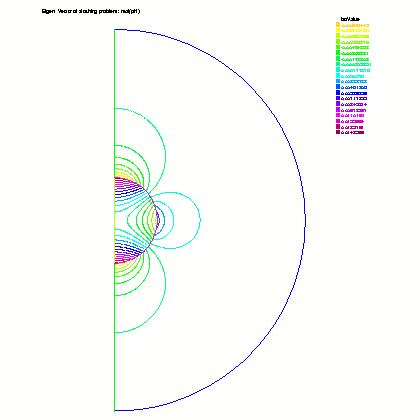
\includegraphics[width=6cm]{3_3_1_potentiel_de_vitesse_2.jpeg}
\caption{potentiel de vitesse $\omega_2$}
%\label{fig:side:a}
\end{minipage}
\begin{minipage}[!htbp]{0.5\linewidth}
\centering
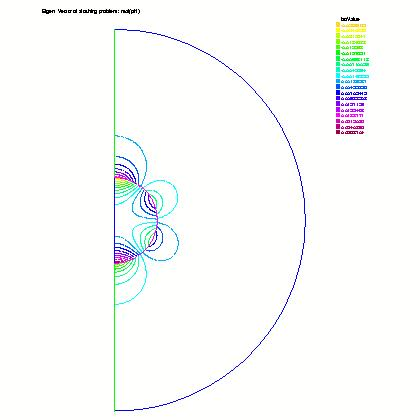
\includegraphics[width=6cm]{3_3_1_potentiel_de_vitesse_3.jpeg}
\caption{potentiel de vitesse $\omega_3$}
%\label{fig:side:b}
\end{minipage}
\end{figure}
\begin{figure}
\begin{minipage}[!htbp]{0.5\linewidth}
\centering
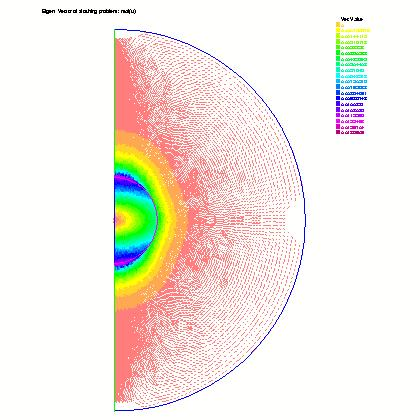
\includegraphics[width=6cm]{3_3_1_champ_de_vitesse_2.jpeg}
\caption{champ de vitesse $\omega_2$}
%\label{fig:side:a}
\end{minipage}
\begin{minipage}[!htbp]{0.5\linewidth}
\centering
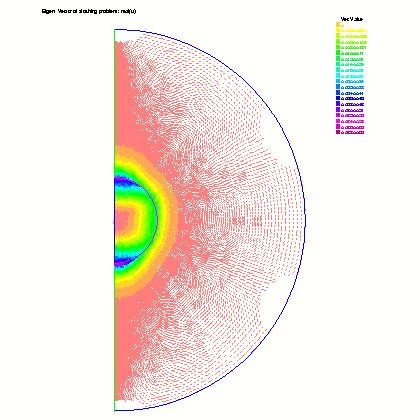
\includegraphics[width=6cm]{3_3_1_champ_de_vitesse_3.jpeg}
\caption{champ de vitesse $\omega_3$}
%\label{fig:side:b}
\end{minipage}
\end{figure}
%%%%%%%%%%%%%%%%%%%%%%%%%%%%%%%%%%%%%%%%%%%%%%%%%%%%
\newpage
\subsection{Cas avec contrainte}
Pour comparer les données expérimentales de Abi Chebel, F. Risso et O. Masbernat,, une goutte attachée à un tube capillaire, on coupe le ligne surface au fond et défini une condition limite que le déplacement de $dl$ est nul. On suppose que la goutte est tenue par une "point" de longueur $dl$ (correspond à cas $\theta = \pi$ de l'étude de chapitre précédent).
%\begin{center}
%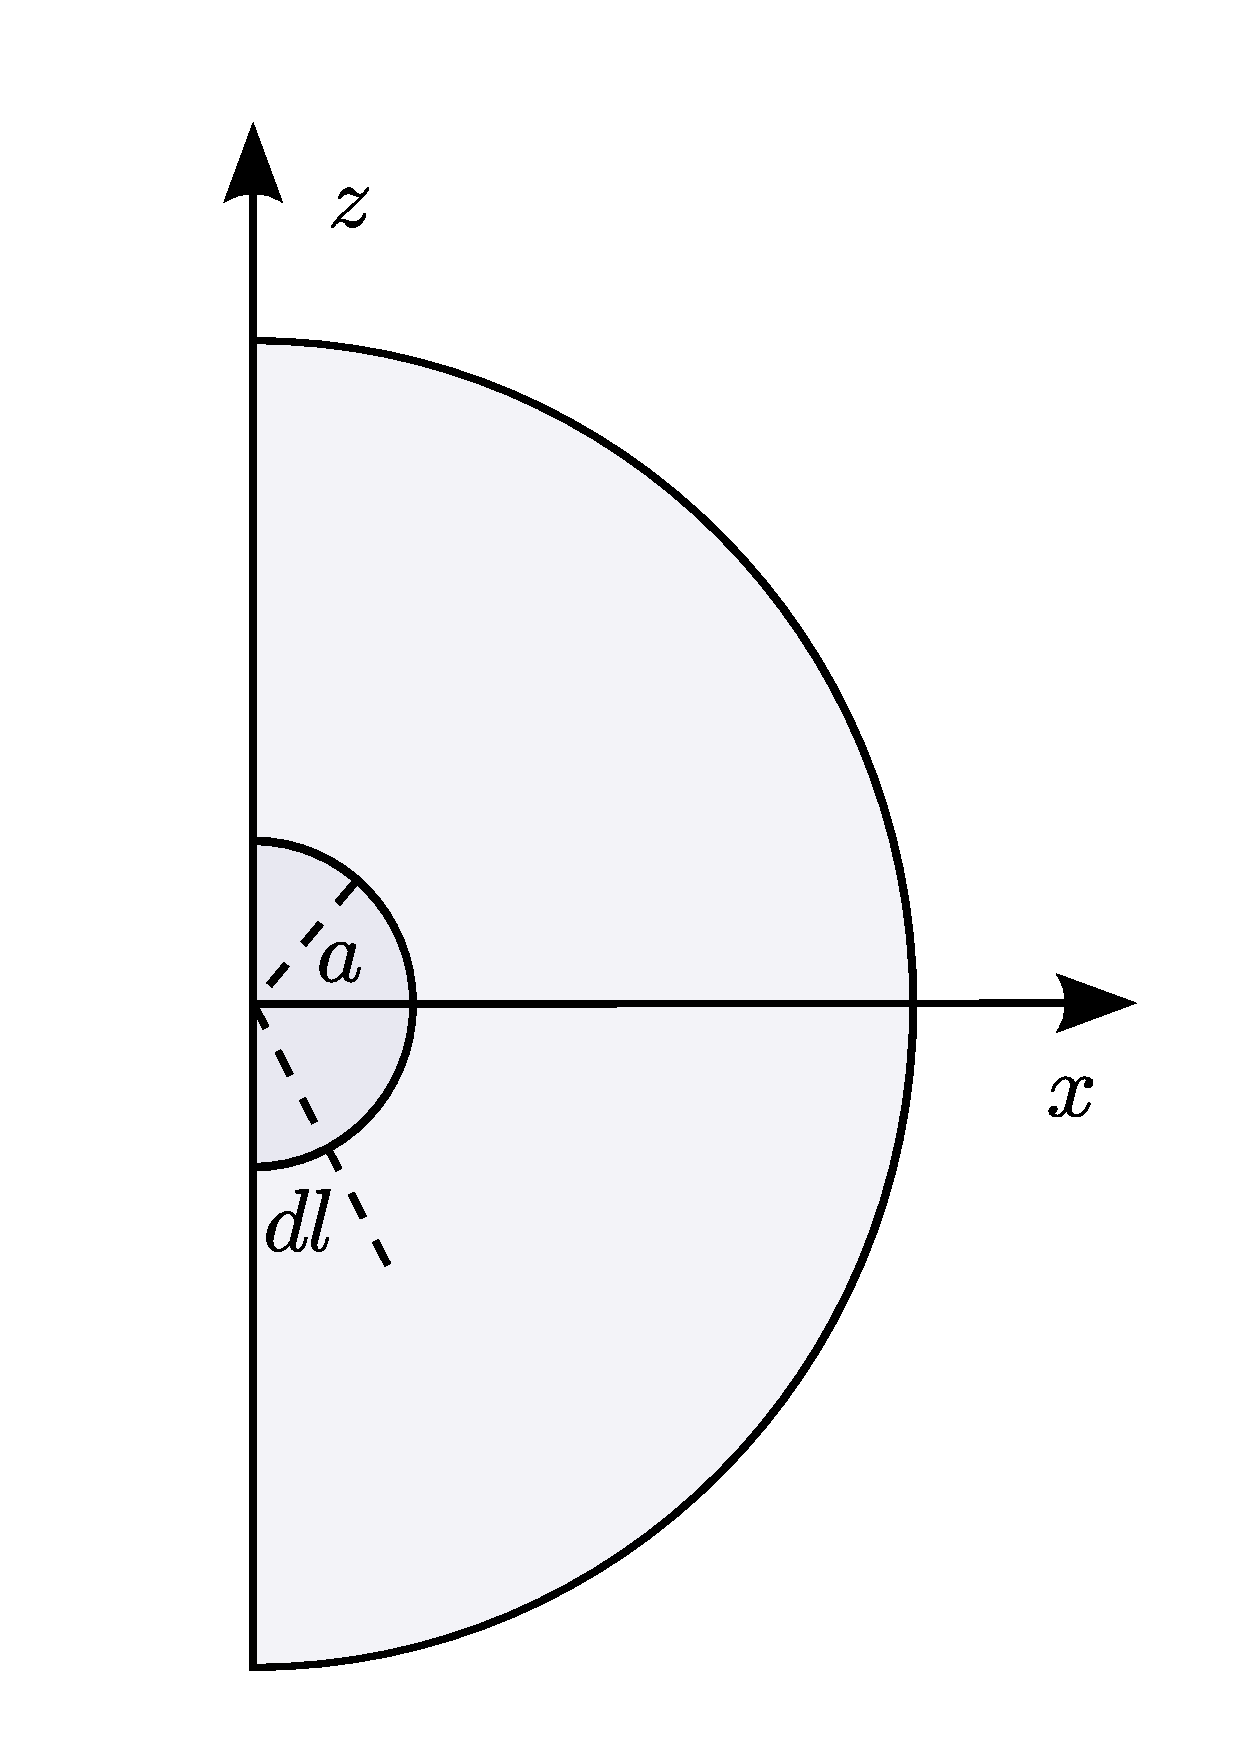
\includegraphics[width=4cm]{3_3_2_mesh}
%\end{center}
\begin{figure}[!htbp]
\centering
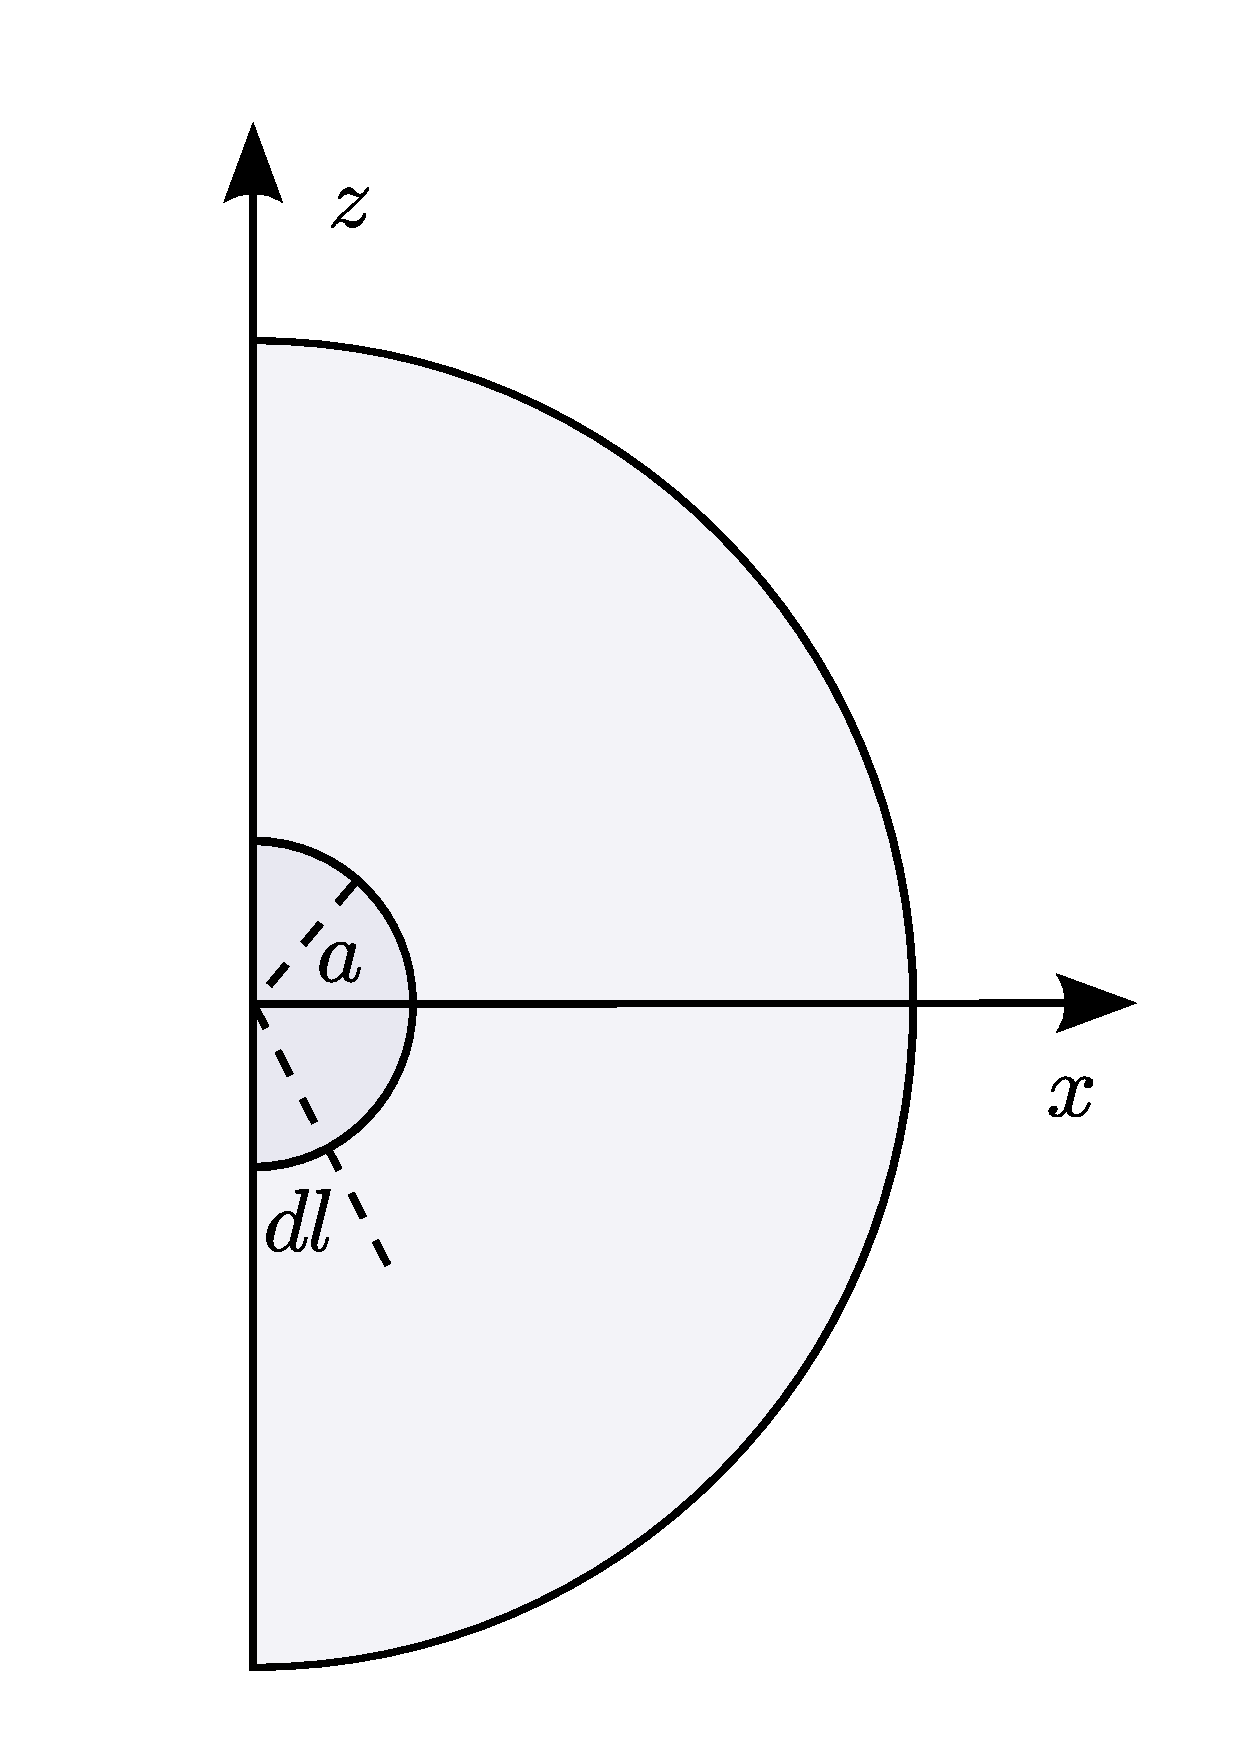
\includegraphics[width=4cm]{3_3_2_mesh}
\caption{Le champ de base d'une goutte avec contrainte dans l'eau}
%\label{fig_res}
\end{figure}
\\[0.25cm]
On va étudier la relation entre la longueur de contrainte $dl$ et la mode du goutte.
\subsubsection{Dans les cas $2a = d = 4.19 mm :$}


\begin{table}[htp]
\begin{center}
    \begin{tabular}{ | l | l | l | l | l | l | }
    \hline
    \multicolumn{2}{|c|}{Mode}  & $\omega_2/2\pi$(Hz) & $\omega_3/2\pi$(Hz) & $\omega_4/2\pi$(Hz) \\
    \hline
    $dl = 0.1$    & $N = 10883$ & 31.3                & 56.6                & 84.9 \\
    \hline
    $dl = 0.01$   & $N = 10659$ & 29.8                & 54.6                & 82.4 \\
    \hline
    $dl = 0.001$  & $N = 10727$ & 29.6                & 54.3                & 82.0 \\
    \hline
    $dl = 0.0004$ & $N = 10899$ & 29.6                & 54.3                & 82.0 \\
    \hline
    $dl = 0.0001$ & $N = 10863$ & nul                 & nul                 & nul \\
    \hline
    \end{tabular}
\end{center}
\caption{Modes deux, trois et quatre d'une goutte avec contrainte dans l'eau pour les cas $2a = d = 4.19 mm :$}
\end{table}
Avec $N$ le nombre de triangles constituant le maillage.
\newpage
\subsubsection{Dans les cas $2a = d = 4.48 mm :$}
\begin{table}[htp]

\begin{center}
    \begin{tabular}{ | l | l | l | l | l | l | }
    \hline
    \multicolumn{2}{|c|}{Mode}  & $\omega_2/2\pi$(Hz) & $\omega_3/2\pi$(Hz) & $\omega_4/2\pi$(Hz) \\
    \hline
    $dl = 0.1$    & $N = 10772$ & 28.2                & 51.1                & 76.7 \\
    \hline
    $dl = 0.01$   & $N = 10678$ & 26.9                & 49.4                & 74.5 \\
    \hline
    $dl = 0.001$  & $N = 10578$ & 26.8                & 49.1                & 74.2 \\
    \hline
    $dl = 0.0004$ & $N = 10606$ & 26.7                & 49.1                & 74.2 \\
    \hline
    $dl = 0.0001$ & $N = 10642$ & nul                 & nul                 & nul \\
    \hline
    \end{tabular}
\end{center}
\caption{Modes deux, trois et quatre d'une goutte avec contrainte dans l'eau pour les cas $2a = d = 4.48 mm :$}
\end{table}
Avec $N$ le nombre de triangles constituant le maillage.



%%%%%%%%%%%%%%%%%%%%%%%%%%%%%%%%%%%%%%%%%%%%%%%%%%%%%%%%%%%%%%%%%%%%%%%%%%%%%%%%%%%%%%%%%%%%%%%%%%%%%%%%%
%%%%%%%%%%%%%%%%%%%%%%%%%%%%%%%%%%%%%%%%%%%%%%%%%%%%%%%%%%%%%%%%%%%%%%%%%%%%%%%%%%%%%%%%%%%%%%%%%%%%%%%%%
%%%%%%%%%%%%%%%%%%%%%%%%%%%%%%%%%%%%%%%%%%%%%%%%%%%%%%%%%%%%%%%%%%%%%%%%%%%%%%%%%%%%%%%%%%%%%%%%%%%%%%%%%
\chapter{Une goutte attachée à un tube capillaire non visqueux}
Dans ce chapitre, on va chercher les modes d'une goutte heptane attachée à un tube capillaire dans l'eau, où la rayon du tube est $1.2mm$. Dans ce but, il faut reconstruire le maillage, redéfinir la courbure, de plus, ajouter les effets de la gravité.
\begin{figure}[!htbp]
\begin{center}
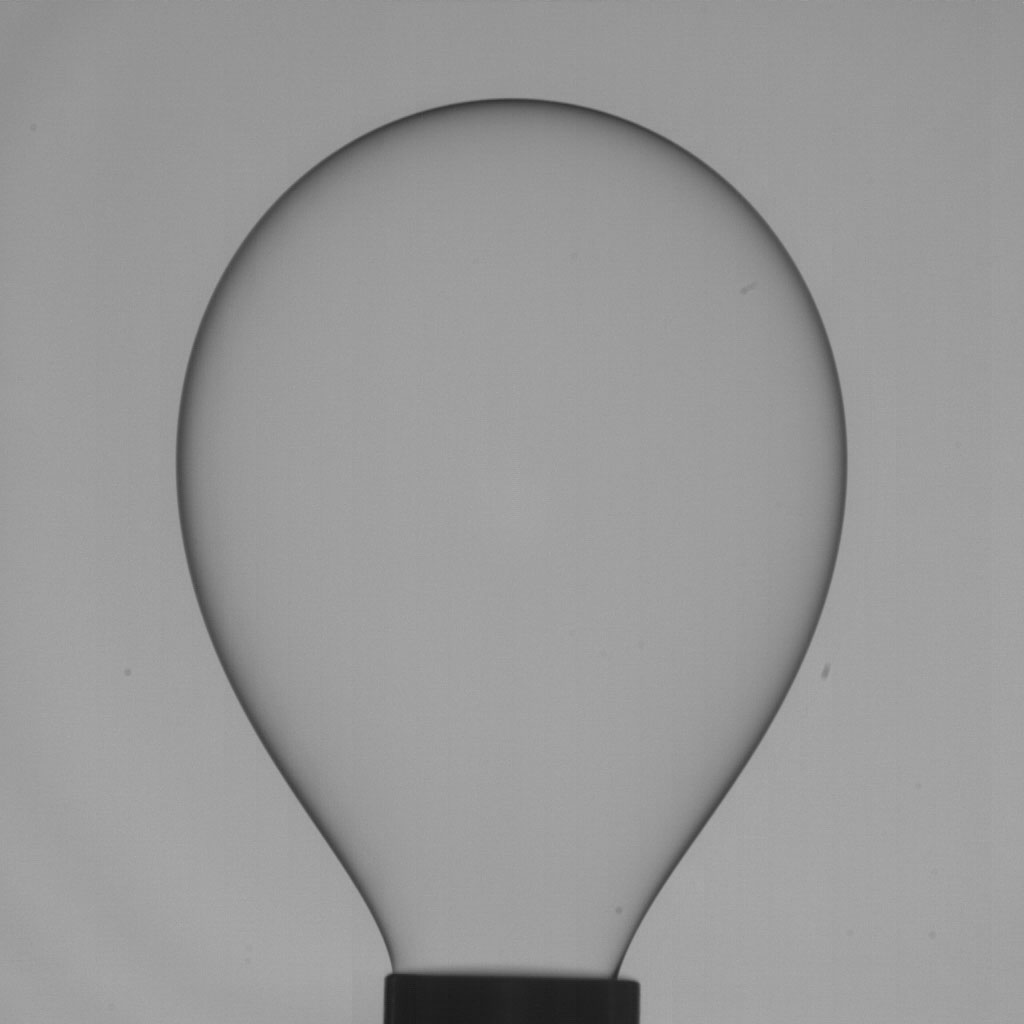
\includegraphics[width=0.6\textwidth, bb = 0 0 1024 1024]{HeptaneWaterApproxGamma_45.jpg}
\caption{Image d'une goutte heptane attachée à un tube capillaire dans l'eau, $\sigma\approx40\ [\frac{mN}{m}]$. G.J. Oosterbaan \cite{6}}
%\label{fig: ImageHeptaneWaterApprox40}
\end{center}
\end{figure}
\newpage
%%%%%%%%%%%%%%%%%%%%%%%%%%%%%%%%%%%%%%%%%%%%%%%%%%%%%%%%%%%%%%%%%%%%%%%%%%%%%%%%%%%%%%%%%%%%%%%%%%%%%%%%%
\section{Position du problème}
%%%%%%%%%%%%%%%%%%%%%%%%%%%%%%%%%%%%%%%%%%%%%%%%%%%%
\subsection{Étude du champ de base}
La première difficulté est de calculer le champ de base, c'est-à-dire la forme d'équilibre de la bulle. Celle-ci est solution l'équilibre de Laplace :
\begin{equation}
K = \Delta P% \quad \text{}
\end{equation}
avec $K$ la courbure et
$$
\Delta P = \Delta P_0 + \Delta \rho g z
$$
Ici $\Delta P_b$ est la différence de pression à la base de la bulle ($z=0$), que l'on impose dans le calcul.\\
\\
Une méthode itérative pour résoudre cette équation est présenté dans l'annexe \ref{Newton}.
%\begin{center}
%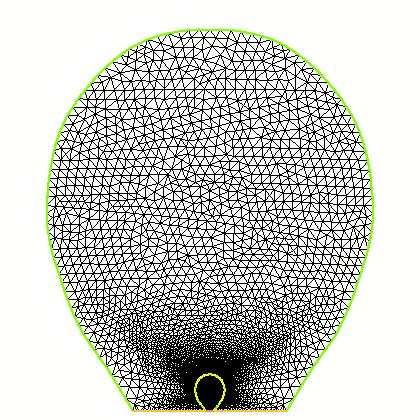
\includegraphics[width=8cm]{4_1_1}
%\end{center}
\begin{figure}[h!] 
\begin{center}
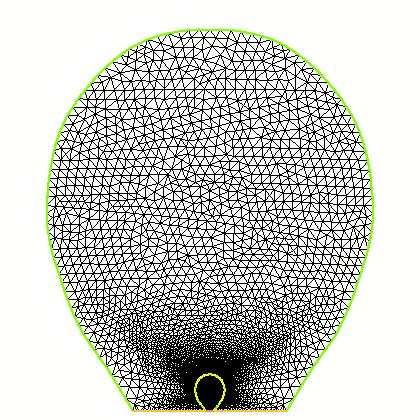
\includegraphics[width=8cm]{4_1_1}
\caption{Le champ de base pour une une goutte dans l'eau}
\label{}
\end{center}
\end{figure}
\\
Nous adopterons le système de coordonnées cylindriques $(r,\theta,z)$.
\begin{tabbing}
Notons :\\
%$a$\,\    \= : le rayon d'équilibre de la goutte\\
$\varPhi_1$ \= : le potentiel de vitesse du fluide 1\\
$\varPhi_2$ \> : le potentiel de vitesse du fluide 2\\
$P_1$       \> : la pression du côté intérieur du fluide 1\\
$P_2$       \> : la pression du côté intérieur du fluide 2
%$H$         \> : le rayon de la goutte
\end{tabbing}
\newpage
On zoome l'image de la goutte comme figure \ref{zoom} :
\begin{figure}[h!] 
\begin{center}
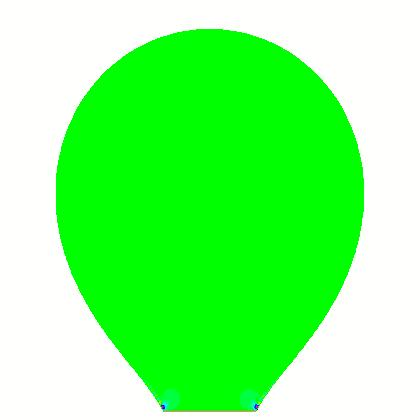
\includegraphics[width=6cm]{4_1_1_zoom}
\caption{Zoom de la figure de la goutte}
\label{zoom}
\end{center}
\end{figure}
%On zoome l'image de la goutte comme au-dessous :
%\begin{center}
%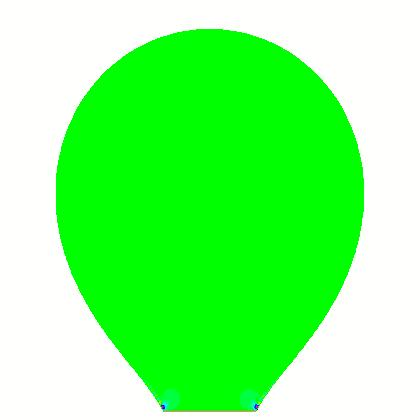
\includegraphics[width=6cm]{4_1_1_zoom}
%\end{center}
%%%%%%%%%%%%%%%%%%%%%%%%%%%%%%%%%%%%%%%%%%%%%%%%%%%%
\subsection{Équations générales}
\begin{eqnarray}\label{pb:41}         %方程组开始
\left\{                              %方程组的左边包括大括号\{
\begin{array}{lll}                   %设定列阵的格式:{lll}是三个L,表示三列的对齐方式为Left对齐
\Delta \varPhi_1 = 0                                                                                     & \text{dans le volume $\Omega_1$}    \\%&——分隔列的标记,\\——表示换行
\Delta \varPhi_2 = 0                                                                                     & \text{dans le volume $\Omega_2$}    \\%&——分隔列的标记,\\——表示换行
P_1 + \rho_1\ \frac{\partial}{\partial t}\varPhi_1 = 0                                                   & \text{dans le volume $\Omega_1$}    \\%&同上
P_2 + \rho_2\ \frac{\partial}{\partial t}\varPhi_2 = 0                                                   & \text{dans le volume $\Omega_2$}    \\%&同上
\frac{\partial}{\partial t} H = \nabla \varPhi_1 \cdot \vec{n} = \frac{\partial}{\partial r} \varPhi_1   & \text{sur la surface libre $S$ (Condition cinématique)}      \\
\frac{\partial}{\partial t} H = - \nabla \varPhi_2 \cdot \vec{n} = - \frac{\partial}{\partial r} \varPhi_2   & \text{sur la surface libre $S$ (Condition cinématique)}      \\
P_2 - P_1 + \Delta{\rho}gz = \sigma\ K                              & \text{sur la surface libre $S$ (Condition dynamique)}   \\% \mathcal{C} ou \mathscr{C}
\text{+ Condition à limite pour la vitesse au fond de la goutte est nul} 
\end{array}                          %方程列阵的结束
\right.                              %方程组的右边无符号,利用“.“来标示
\end{eqnarray}                       %方程组结束
\begin{flalign*}
\text{où}   & &\\
\sigma      &: \text{le coefficient de tension superficielle} &\\
K           &: \text{la courbure moyenne de l'interface} &\\
\Delta{\rho}&= P_2 - P_1 &
\end{flalign*}
%%%%%%%%%%%%%%%%%%%%%%%%%%%%%%%%%%%%%%%%%%%%%%%%%%%%
\newpage
\subsection{Décomposition modale}
On considère maintenant l'oscillation linéaire d'une goutte par rapport à la position d'équilibre :
\begin{eqnarray*}
\varPhi_1   &=& \varPhi_{10} + \varphi_1(r,\theta,z)\ e^{- i \omega t} \\
\varPhi_2   &=& \varPhi_{20} + \varphi_2(r,\theta,z)\ e^{- i \omega t} \\
P_1         &=& P_{10} + p_1(r,\theta,z)\ e^{- i \omega t}\\
P_2         &=& P_{20} + p_2(r,\theta,z)\ e^{- i \omega t}
%H           &=& a + \varepsilon\ \eta(\theta,\phi)\ e^{- i \omega t}
\end{eqnarray*}
\begin{center}
\includegraphics[width=10cm, angle=270]{5}
\end{center}
On suppose que la forme moyenne de l'interface est donnée par un paramétrage de la forme $M_0(s_0)$, où $s_0$ est l'abscisse curviligne associée. On note $T_0$, $N_0$, $K_0$ les vecteurs tangents, normal, et la courbure associée. Ceux-ci sont donnés par :
\\[0.25cm]
$$
{\bf T}_0 = \frac{\partial \vec{OM_0}}{\partial s_0}
$$
\\[0.25cm]
\begin{equation*}
K_0 = K_0^{(a)} + K_0^{(b)} = {\bf T_0} \cdot \frac{\partial {\bf N}_0}{\partial s_0} + \frac{{\bf N}_{0,r}}{r}
\end{equation*}
\\[0.25cm]
On suppose maintenant que la surface oscille faiblement autour de la forme moyenne précédemment définie (voir figure b).
\newpage
On choisit de paramétrer la déformation de la manière suivante :
\\[0.25cm]
$$
\vec{OM}(s_0)  = \vec{OM_0}(s_0) + \varepsilon \eta(s_0) {\bf N}_0\ e^{- i \omega t}
$$
\\[0.25cm]
D'après le travail de D. Fabre,  \emph{Calcul de la courbure} joint dans la Annexes, on sait que
\\[0.25cm]
$$
K = K_0 + \varepsilon K_1
$$
où
\\[0.25cm]
$$
K_0   = {\bf T_0} \frac{\partial \bf N_0}{\partial s_0}  + \frac{N_{0,r}}{r}
$$
\\[0.25cm]
$$
K_1   =
- \left[\
\frac{1}{r} \frac{\partial }{\partial s_0} \left( r \frac{\partial \eta}{\partial s_0} \right)
+
\left( \left| \frac{\partial \bf N_0}{\partial s_0} \right|^2  + \frac{N_{0,r}^2}{r^2} \right) \eta
\ \right]\ e^{- i \omega t}.
$$
%%%%%%%%%%%%%%%%%%%%%%%%%%%%%%%%%%%%%%%%%%%%%%%%%%%%
\subsection{Linéarisation des équations}
La linéarisation des équations s'effectue en remplaçant dans le système d'équations d'équilibre \eqref{pb:41} le potentiel de vitesse, le champ de pression et la courbure par leur décomposition, puis en conservant uniquement les termes d'ordre 1 par rapport aux petites perturbation introduites. Nous obtenons ainsi le problème linéaire suivant :
\begin{eqnarray}\label{pb:42}         %方程组开始
\left\{                              %方程组的左边包括大括号\{
\begin{array}{lll}                   %设定列阵的格式:{lll}是三个L,表示三列的对齐方式为Left对齐
\Delta \varphi_1 = 0                                                                                     & \text{dans le volume $\Omega_1$}    \\%&——分隔列的标记,\\——表示换行
\Delta \varphi_2 = 0                                                                                     & \text{dans le volume $\Omega_2$}    \\%&——分隔列的标记,\\——表示换行
p_1 + \lambda\ \rho_1\ \varphi_1 = 0                                                                     & \text{dans le volume $\Omega_1$}    \\%&同上
p_2 + \lambda\ \rho_2\ \varphi_2 = 0                                                                     & \text{dans le volume $\Omega_2$}    \\%&同上
\lambda\ \eta = \nabla \varphi_1 \cdot \vec{n} = \frac{\partial}{\partial r} \varphi_1                   & \text{sur la surface libre $S$}      \\
\lambda\ \eta = - \nabla \varphi_2 \cdot \vec{n} = - \frac{\partial}{\partial r} \varphi_2               & \text{sur la surface libre $S$}      \\
p_2 -p_1 + \Delta{\rho} g \eta \cdot \vec{e}_z = - \sigma\ \left[\
\frac{1}{r} \frac{\partial}{\partial s_0} \left( r \frac{\partial \eta}{\partial s_0} \right)
+
\left( \left| \frac{\partial \bf N_0}{\partial s_0} \right|^2  + \frac{N_{0,r}^2}{r^2} \right) \eta
\ \right]                                                                                                & \text{sur la surface libre $S$}   % \mathcal{C} ou \mathscr{C}
\end{array}                          %方程列阵的结束
\right.                              %方程组的右边无符号,利用“.“来标示
\end{eqnarray}                       %方程组结束
Avec $\lambda = - i \omega t$ les valeurs propre recherchés.
%%%%%%%%%%%%%%%%%%%%%%%%%%%%%%%%%%%%%%%%%%%%%%%%%%%%%%%%%%%%%%%%%%%%%%%%%%%%%%%%%%%%%%%%%%%%%%%%%%%%%%%%%
\newpage
\section{Modélisation numérique}
%%%%%%%%%%%%%%%%%%%%%%%%%%%%%%%%%%%%%%%%%%%%%%%%%%%%
\subsection{Formulation variationnelle}
Pour l'implémentation de ces équations sous FreeFem++ il convient de mettre en place une formulation variationnelle (ou formulation faible). Pour cela, introduit des fonction test $\varphi^*_1, \varphi^*_2, p^*_1, p^*_2, \eta^*$ associées à $\varphi_1, \varphi_2, p_1, p_2, \eta$, où $(\varphi^*_1, p^*_1)$ définis sur $\Omega_1$, $(\varphi^*_2, p^*_2)$ définis sur $\Omega_2$, $\eta^*$ défini sur $S$.
\\[0.25cm]
Comme nous l'avons vu au chapitre précédent, on déduit la formulation variationnelle du problème \eqref{pb:42} :
\\[0.25cm]
$\forall \varphi^*_1, \varphi^*_2, p^*_1, p^*_2, \eta^*$,
\begin{eqnarray}\label{pb:43}
\left\{
\begin{array}{rcl}
(\ \nabla \varphi_1 ,\ \nabla \varphi^*_1 \ )_{\Omega_1} &=& \lambda\ <\ \eta,\ \varphi^*_1 \ >_S \\
- (\ p_1 ,\ p^*_1 \ )_{\Omega_1} &=& \lambda\ (\ \rho_1\ \varphi_1 ,\ p^*_1 \ )_{\Omega_1} \\
(\ \nabla \varphi_2 ,\ \nabla \varphi^*_2 \ )_{\Omega_2} &=& - \lambda\ <\ \eta,\ \varphi^*_2 \ >_S \\
- (\ p_2 ,\ p^*_2 \ )_{\Omega_2} &=& \lambda\ (\ \rho_2\ \varphi_2 ,\ p^*_2 \ )_{\Omega_2} \\
<\ p_2 - p_1 + \Delta{\rho} g \eta \cdot \vec{e}_z + \sigma\ \left[\
\frac{1}{r} \frac{\partial}{\partial s_0} \left( r \frac{\partial \eta}{\partial s_0} \right)
+
\left( \left| \frac{\partial \bf N_0}{\partial s_0} \right|^2  + \frac{N_{0,r}^2}{r^2} \right) \eta
\ \right] ,\ \eta^* \ >_S &=& 0
\end{array}
\right.
\end{eqnarray}
On sait que
\begin{eqnarray*}
<\ \sigma\ \frac{1}{r} \frac{\partial}{\partial s_0} \left( r \frac{\partial \eta}{\partial s_0} \right) ,\ \eta^* \ >_S
=
- <\ \sigma\ \frac{\partial}{\partial s_0} \eta ,\ \frac{\partial}{\partial s_0} \eta* \ >_S
\end{eqnarray*}
On peux simplifie la formulation \eqref{pb:43} comme la forme suivante :
\begin{eqnarray}\label{pb:44}
\left\{
\begin{array}{rcl}
(\ \nabla \varphi_1 ,\ \nabla \varphi^*_1 \ )_{\Omega_1} &=& \lambda\ <\ \eta,\ \varphi^*_1 \ >_S \\
- (\ p_1 ,\ p^*_1 \ )_{\Omega_1} &=& \lambda\ (\ \rho_1\ \varphi_1 ,\ p^*_1 \ )_{\Omega_1} \\
(\ \nabla \varphi_2 ,\ \nabla \varphi^*_2 \ )_{\Omega_2} &=& - \lambda\ <\ \eta,\ \varphi^*_2 \ >_S \\
- (\ p_2 ,\ p^*_2 \ )_{\Omega_2} &=& \lambda\ (\ \rho_2\ \varphi_2 ,\ p^*_2 \ )_{\Omega_2} \\
<\ p_2 - p_1 + \Delta{\rho} g \eta \cdot \vec{e}_z + \sigma\ \left( \left| \frac{\partial \bf N_0}{\partial s_0} \right|^2  + \frac{N_{0,r}^2}{r^2} \right) \ \eta ,\ \eta^* \ >_S - <\ \sigma\ \frac{\partial}{\partial s_0} \eta ,\ \frac{\partial}{\partial s_0} \eta* \ >_S &=& 0 \\
\text{+ Condition à limite pour la vitesse au fond de la goutte est nul} 
\end{array}
\right.
\end{eqnarray}
%%%%%%%%%%%%%%%%%%%%%%%%%%%%%%%%%%%%%%%%%%%%%%%%%%%%
\subsection{Écriture du problème sous forme matricielle}
On peut met la formulation variationnelle \eqref{pb:44} sous la forme matricielle suivante :
\begin{equation}\label{eq:45}
\begin{bmatrix}
A_{11} & 0      & 0      & 0      & 0\\
0      & A_{22} & 0      & 0      & 0\\
0      & 0      & A_{33} & 0      & 0\\
0      & 0      & 0      & A_{44} & 0\\
0      & A_{52} & 0      & A_{54} & A_{55}
\end{bmatrix}
=
\lambda
\begin{bmatrix}
0      & 0 & 0      & 0 & B_{15}\\
B_{21} & 0 & 0      & 0 & 0\\
0      & 0 & 0      & 0 & B_{35}\\
0      & 0 & B_{43} & 0 & 0\\
0      & 0 & 0      & 0 & 0
\end{bmatrix}
\end{equation}
%%%%%%%%%%%%%%%%%%%%%%%%%%%%%%%%%%%%%%%%%%%%%%%%%%%%%%%%%%%%%%%%%%%%%%%%%%%%%%%%%%%%%%%%%%%%%%%%%%%%%%%%%
\newpage
\section{Validation du code}
%%%%%%%%%%%%%%%%%%%%%%%%%%%%%%%%%%%%%%%%%%%%%%%%%%%%
\subsection{Dans les cas $2a = d = 4.19 mm :$}

\begin{table}[htp]
\begin{center}
    \begin{tabular}{ | l | l | l | l | l | }
    \hline
    Mode & $\omega_2/2\pi$(Hz) & $\omega_3/2\pi$(Hz) & $\omega_4/2\pi$(Hz) \\
    \hline
    $N = 8290$    & 30.9 & 56.2 & 85.0 \\ %10
    \hline
    $N = 19070$   & 30.7 & 56.0 & 83.9 \\ %20
    \hline
    $N = 36240$   & 30.6 & 55.8 & 84.0 \\ %30
    \hline
    \end{tabular}
\end{center}
     \caption{Modes deux, trois et quatre d'une goutte attachée}
\end{table}
Avec $N$ le nombre de triangles constituant le maillage.
%%%%%%%%%%%%%%%%%%%%%%%%%%%%%%%%%%%%%%%%%%%%%%%%%%%%
\subsection{Dans les cas $2a = d = 4.48 mm :$}
C'est un cas que la forme est critique éclatement, on ne construit pas le maillage par la méthode joint dans la Annexes.
\subsection{Comparaison}
Ensuite on étude les modes en comparaison avec le cas d'une goutte libre.


\begin{table}[htp]
\begin{center}
    \begin{tabular}{ | l || l | l | l || l | l | l || l | l | l || }
    \hline
    Mode          &\multicolumn{3}{c||}{$\omega_2/2\pi$(Hz)} & \multicolumn{3}{c||}{$\omega_3/2\pi$(Hz)} & \multicolumn{3}{c||}{$\omega_4/2\pi$(Hz)} \\
    \hline
                  & Attachée & Libre & Contrainte & Attachée & Libre & Contrainte & Attachée & Libre & Contrainte \\
    \hline
    $N = 18797$   &          & 27.7  &            &          & 52.1  &            &          &79.5   &            \\
    \hline
    $N = 29706$   &          & 27.7  &            &          & 52.1  &            &          &79.4   &            \\
    \hline
    $N = 10863$   &          &       & 29.6       &          &       & 54.3       &          &       & 82.0       \\
    \hline
    $N = 19070$   & 30.7     &       &            & 56.0     &       &            & 83.9     &       &            \\
    \hline
    $N = 36240$   & 30.6     &       &            & 55.8     &       &            & 84.0     &       &            \\
    \hline
    \end{tabular}
\end{center}
\caption{Comparaison des modes d'une goute attachée, libre, contrainte dans les cas $2a = d = 4.48 mm :$}
\end{table}



Avec $N$ le nombre de triangles constituant le maillage.

















































%%%%%%%%%%%%%%%%%%%%%%%%%%%%%%%%%%%%%%%%%%%%%%%%%%%%%%%%%%%%%%%%%%%%%%%%%%%%%%%%%%%%%%%%%%%%%%%%%%%%%%%%%
%%%%%%%%%%%%%%%%%%%%%%%%%%%%%%%%%%%%%%%%%%%%%%%%%%%%%%%%%%%%%%%%%%%%%%%%%%%%%%%%%%%%%%%%%%%%%%%%%%%%%%%%%
%%%%%%%%%%%%%%%%%%%%%%%%%%%%%%%%%%%%%%%%%%%%%%%%%%%%%%%%%%%%%%%%%%%%%%%%%%%%%%%%%%%%%%%%%%%%%%%%%%%%%%%%%
\chapter{Conclusion}

Pour conclure, un code FreeFem++ permettant d'effectuer une étude de stabilité globale d'une goutte a été implémenté.
Ce code a été validé tout d'abord dans le cas d'une goutte libre et le cas d'une goutte avec contrainte qui oscille tout en étant tenue par un anneau circulaire,
puis pour une goutte de liquide immergée dans un autre fluide.
\\[0.25cm]
Mais pour les cas d'une goutte attachée à un tube capillaire, la précision des résultats ne suffit pas vérifier les conclusion de N. Abi Chebel, F. Risso et O. Masbernat \cite{3}.
Cependant un résultat intéressant est de constater que les fréquences d'oscillation d'une goutte attachée de forme non sphérique sont en bon accord avec celles d'une goutte sphérique avec une contrainte en un point. Un limitation de notre étude est le caractère non visqueux de celle-ci. Pour faire une comparaison plus rigoureuse avec l'expérience, il serait souhaitable d'inclure l'effet de la viscosité. Par cela on peut posséder en deux étapes : 
\\[0.25cm]
1 ) Garder l'hypothèse de l'écoulement potentiel et ne tenir compte que de la viscosité de volume.\\
2 ) Prendre en compte également l'effet des couches limites ce qui nécessite de modifier la formulation variationnelle.
\\[0.25cm]
Enfin, on a constaté que la méthode mise en place pour calculer la forme moyenne de la goutte ne converge pas toujours, ce point est également à améliorer.








%%%%%%%%%%%%%%%%%%%%%%%%%%%%%%%%%%%%%%%%%%%%%%%%%%%%%%%%%%%%%%%%%%%%%%%%%%%%%%%%%%%%%%%%%%%%%%%%%%%%%%%%%
%%%%%%%%%%%%%%%%%%%%%%%%%%%%%%%%%%%%%%%%%%%%%%%%%%%%%%%%%%%%%%%%%%%%%%%%%%%%%%%%%%%%%%%%%%%%%%%%%%%%%%%%%
%%%%%%%%%%%%%%%%%%%%%%%%%%%%%%%%%%%%%%%%%%%%%%%%%%%%%%%%%%%%%%%%%%%%%%%%%%%%%%%%%%%%%%%%%%%%%%%%%%%%%%%%%
\chapter{Annexes : Calcul de la courbure}
%%%%%%%%%%%%%%%%%%%%%%%%%%%%%%%%%%%%%%%%%%%%%%%%%%%%%%%%%%%%%%%%%%%%%%%%%%%%%%%%%%%%%%%%%%%%%%%%%%%%%%%%%
Ce sont les travaux de D. Fabre.
\section{Formules de base}
\begin{figure}[!htbp]
\centering
\includegraphics[width=10cm, angle=270]{5}
\caption{champ de vitesse}
%\label{fig_res}
\end{figure}
On cherche a exprimer la courbure d'une surface ayant une symétrie de révolution.\\
La courbure $K$ se décompose en deux termes :
$$
K = K^{(a)} + K^{(b)} 
\quad \mbox{ avec }  
\left| K^{(a)} \right|  = \frac{1}{| MC^{(a)} |} 
\quad \mbox{ et } 
\left| K^{(b)} \right| =  \frac{1}{| MC^{(b)} | }
$$
Le premier terme est la courbure dans le plan méridien ; géométriquement, on l'exprime avec le point  $C^{(a)}$ qui est le centre du cercle osculateur à la courbe méridienne. Le second terme est la courbure dans le plan orthogonal ; on l'exprime avec le point $C^{(b)}$ qui est l'intersection entre la normale à la courbe et l'axe de symétrie (voir figure a).\\
On prend la convention suivante pour le signe de $K^{(a)}$ et  $K^{(b)}$ :
celles-ci sont positives si la surface est convexe et négatives si la surface est concave. Par exemple, dans le cas représenté sur la figure, on a $K^{(a)}>0$ et  $K^{(b)}<0$.
\\
Le premier terme se calcule a partir des formules de Frénet. On suppose que la courbe méridienne, dans le plan $(r,z)$, admet une représentation paramètrique $M(s)$, où $s$ est l'abscisse curviligne. On note $\bf T$ le vecteur tangent à la courbe dans le plan méridien, et $\bf N$ le vecteur normal. On a :
$$
{\bf T} = \DP{\vec{OM}}{s}
$$
$$
\DP{{\bf T}}{s} = - K^{(a)} {\bf N}
$$
$$
\DP{{\bf N}}{s} = K^{(a)} {\bf T}
$$
En pratique on peut aussi utiliser la formule suivante :
$$
K^{(a)} =  {\bf T} \cdot \DP{{\bf N}}{s} =   {\bf T} \cdot (\nabla {\bf N}) \cdot {\bf T} 
$$
Le second terme a l'expression suivante :
$$
K^{(b)} =  \frac{ N_{,r}}{r}
$$
où $N_{,r} = {\bf N} \cdot {\bf e_r}$ est la composante radiale du vecteur normal.
\section{Courbure de la forme moyenne}
On suppose que la forme moyenne de l'interface est donnée par un paramètrage de la forme $M_0(s_0)$, où $s_0$ est l'abscisse curviligne associée. On note $T_0$, $N_0$, $K_0$ les vecteurs tangents, normal, et la courbure associée. Ceux-ci sont donnés par :
$$
{\bf T}_0 = \DP{\vec{OM_0}}{s_0}
$$
\begin{equation}
K_0 = K_0^{(a)} + K_0^{(b)} =  {\bf T_0} \cdot \DP{{\bf N}_0}{s_0} 
+ \frac{{\bf N}_{0,r}}{r}
\end{equation}
\section{Perturbation}
On suppose maintenant que la surface oscille faiblement autour de la forme moyenne précédemment définie (voir figure b).
\\
On choisit de paramètrer la déformation de la manière suivante :
$$
\vec{OM}(s_0)  = \vec{OM_0}(s_0) + \epsilon \eta(s_0) {\bf N}_0
$$
Dans cette expression, $\epsilon$ est un petit paramètre, et la fonction $\eta$ correspond à l'amplitude de la déformation mesurée dans la direction normale à la surface {\em moyenne}. Notons que l'on garde le paramétrage par la variable $s_0$ qui est l'abscisse curviligne de la forme moyenne (et qui n'est pas identique à l'abscisse curviligne $s$ de la surface déformée).
\\
On injecte maintenant ce paramétrage dans les formules précédentes, et on linéarise par rapport à $\epsilon$, ce qui aboutit à :
$$
\DP{s}{s_0} = \left| \DP{\vec{OM}}{s_0} \right| = 1 - \epsilon \eta K_0^{(a)} ;
$$
$$
{\bf T} = \left(\DP{s}{s_0}\right)^{-1} \DP{\vec{OM}}{s_0} = {\bf T}_0 +  \epsilon  {\bf T}_1 ; \quad 
{\bf T}_1 = - \DP{\eta}{s_0}{\bf N_0}
$$
$$
{\bf N} = {\bf N}_0 +  \epsilon  {\bf N}_1 ; \quad 
{\bf N}_1 = \DP{\eta}{s_0}{\bf T_0}
$$
$$
K^{(a)} = {\bf T} \cdot \DP{{\bf N}}{s} =  
\left( {\bf T}_0 +  \epsilon  {\bf T}_1 \right) \left( \DP{s_0}{s} \right) 
 \DP{}{s_0}  \left({\bf N}_0 +  \epsilon  {\bf N}_1 \right)
$$
$$
= K^{(a)}_0 + \epsilon K^{(a)}_1
$$
$$
K^{(a)}_1 = 
-\DP{^2 \eta }{s_0^2} - \left( K^{(a)}_0 \right)^2 \eta 
$$
De même, pour la seconde composante de la courbure :
$$
K^{(b)} = \frac{ N_{,r}}{r} = \frac{ N_{0,r} + \epsilon N_{1,r}}{r + \epsilon \eta N_{0,r}}
$$
$$
= 
K^{(b)}_0 + \epsilon K^{(b)}_1
$$
$$
K^{(b)}_1 = - \frac{T_{0,r}}{r} \DP{\eta}{s_0} -  \left( K^{(b)}_0 \right)^2 \eta 
$$
Au final on a donc :
$$
K = K_0 + \epsilon K_1
$$
$$
K_0   = {\bf T_0} \DP{\bf N_0}{s_0}  + \frac{N_{0,r}}{r}
$$
$$
K_1   = - \frac{1}{r} \DP{}{s_0} \left( r \DP{\eta}{s_0} \right) -
\left[ \left| \DP{\bf N_0}{s_0} \right|^2  + \frac{N_{0,r}^2}{r^2} \right] \eta
$$
Dans cette dernière expression on a utilisé l'identité $T_{0,r} = \partial r / \partial s_0$
\section{Cas particulier : forme moyenne sphérique}
On suppose que la forme moyenne est une sphére de rayon $R_0$. On utilise les coordonnées sphériques $(R,\Theta)$. Dans ce cas, l'abscisse curviligne de la forme moyenne $s_0$ est donné par $s_0  = R_0 \Theta$, et on a :
$$
r = R_0 \sin \Theta ; \quad z = R_0 \cos \Theta; \quad \DP{}{s_0} = \frac{1}{R_0} \DP{}{\Theta}
$$
$$
{\bf N_0} = {\bf e_R} ; \quad {\bf T_0} = {\bf e_\Theta} ; \quad N_{0,r} = \sin \Theta; 
$$
En injectant dans les formules précédentes, on aboutit à :
$$
K_0 = \frac{2}{R_0}
$$
$$ 
K_1 = - \frac{1}{R_0^2 \sin \Theta} \DP{}{\Theta} \left( \sin \Theta \DP{\eta}{\theta} \right) 
- \frac{2}{R_0^2} \eta
$$
Ce qui correspond bien aux formules obtenues dans ce cas.
\section{Paramétrage selon $r$}
Vérifions que les formules générales trouvée ici est équivalente à celles utilisées dans le cas où la surface est paramétrée par $r$ et non par $s_0$ C'est-à-dire :
$$
z = H(r) = h_0(r) + \epsilon \eta_z (r)
$$
Dans ce cas le calcul de la courbure conduit à :
$$
K =  K_0(r) + \epsilon k(r)
$$
avec :
$$
K_0(r) = -\frac{1}{r} \DP{}{r} \left( \frac{r}{\sqrt{1+ h_0'^2}} \DP{h_0}{r} \right)
$$
$$
k(r) = -\frac{1}{r} \DP{}{r} \left( \frac{r}{\left(1+ h_0'^2\right)^3} \DP{\eta_z}{r} \right) 
$$
(Par rapport aux formules données dans le rapport de Jérôme on a changé les signes afin d'utiliser la même convention sur les normales, et on a rectifié une petite erreur dans le terme $k$).
\\
La correspondance entre les deux formulations s'établit en utilisant les identités suivantes :
$$ 
\eta_z(r) = \frac{\eta(s_0)}{N_{0,z}}  ; 
\quad 
T_{0,r} = N_{0,z} = \frac{1}{\sqrt{1+ h_0'^2}}; 
\quad 
T_{0,z} = -N_{0,r} =  \frac{h_0'}{\sqrt{1+ h_0'^2}}
$$
$$
\DP{}{r} = N_{0,z} \DP{}{s_0}
$$
$$
k(r) = K_1(s_0)  - \DP{K_0}{s_0} T_{0,z} \eta_z(r)
$$
(formules vérifiées avec Maple)
\section{Calcul de la forme d'équilibre par méthode de Newton}\label{Newton}
Le but est de construire un maillage tel que le long de sa frontière, on ait l'équilibre de Laplace :
\begin{equation}
F = K - \frac{\Delta P}{\sigma} = 0.
\end{equation}
avec 
$$
\Delta P = \Delta P_b + \Delta \rho g z
$$
Ici $\Delta P_b$ est la différence de pression à la base de la bulle ($z=0$), que l'on impose dans le calcul (on pourrait aussi imposer le volume dans la bulle et considérer $\Delta P_b$ comme une inconnue, mais cela reste à faire proprement).\\
La méthode est la suivante :
\begin{enumerate}
\item On part d'un maillage correspondant à une forme approximative de la bulle (par exemple un développement en série de Legendre issu des expériences).
\item On écrit un développement de Taylor de la fonction $F$ par rapport à des petites variations $\eta$ de la forme de la surface :
$$ 
F \approx F_0 + F_1 = 0 \quad  \mbox{ avec } 
F_0 = K_0 - (\Delta P + \Delta \rho g z)/ \sigma , 
\quad  
F_1 = K_1 - \frac{\Delta \rho g}{\sigma} N_{0,z} \eta
$$
où $K_1$ est donné (en fonction de $\eta$) par la formule de la section précédente.
\item On inverse la relation précédente, ce qui donne la fonction $\eta$ correspondant au déplacement qu'il faut donner à l'interface pour assurer la condition $F=0$ (sous l'hypothèse de linéarisation).
\item On construit un champ de vecteurs $\bf U$, défini à l'intérieur du domaine, correspondant à un déplacement lagrangien vérifiant ${\bf U} = \eta {\bf N_0}$ sur la frontière du domaine et étant suffisamment régulier à l'intérieur (en pratique on résoud une équation de Poisson).
\item On déforme le maillage selon le champ de vecteur $\bf U$, ce qui aboutit à un nouveau maillage en principe plus proche de la solution d'équilibre.
\item On répète l'opération de manière itérative a partir du point ($b$), jusqu'à convergence
(c'est à dire jusqu'à ce que la quantité $F_0$ devienne effectivement négligeable.
\end{enumerate}
\section{Implémentation avec Freefem}
Pour le calcul de la courbure moyenne, il faut commencer par interpoler les vecteurs normal (et tangent) sous forme de champs P1 définis sur la frontière :
\begin{verbatim}
(...)

mesh Shempty=emptymesh(Sh);
fespace Wh1(Shempty,P1);
Wh1 N0r,N0z,T0r,T0z,K0a,K0b,test ;

problem CalcN0r(N0r,test)=
 int1d(Shempty,qfe=qf3pE)(N0r*test)-int1d(Shempty,qfe=qf3pE)(N.x*test);
problem CalcN0z(N0z,test)=
 int1d(Shempty,qfe=qf3pE)(N0z*test)-int1d(Shempty,qfe=qf3pE)(N.y*test);

CalcN0r;
CalcN0z;
T0r =  N0z;
T0z = -N0r;

macro Ds(u1,u2)
[dx(u1)*T0r+dy(u1)*T0z,dx(u2)*T0r+dy(u2)*T0z]
//

problem ComputeK0a(K0a,test)=
 int1d(Shempty,qfe=qf3pE)(K0a*test)
-int1d(Shempty,qfe=qf3pE)(Ds(N0r,N0z)'*[T0r,T0z]*test);
ComputeK0a;

problem ComputeK0b(K0b,test)=
 int1d(Shempty,qfe=qf3pE)(K0b*test*x)
-int1d(Shempty,qfe=qf3pE)(N0r*test);
ComputeK0b;


\end{verbatim}
Pour les perturbations, le terme de courbure se traite par intégration par partie :
$$
p = \sigma K_1 
$$
$$
\int_{\cal S}  \eta^\dag p r d \ell 
 = \sigma 
 \int_{\cal S} \left (
 \DP{\eta^\dag}{s_0} \DP{\eta}{s_0} - \left[ \left| \DP{\bf N_0}{s_0} \right|^2  + \frac{N_{0,r}^2}{r^2} \right]  \eta^\dag \eta \right) r d \ell 
\mbox{ (+ termes de bord)} 
$$



%%%%%%%%%%%%%%%%%%%%%%%%%%%%%%%%%%%%%%%%%%%%%%%%%%%%%%%%%%%%%%%%%%%%%%%%%%%%%%%%%%%%%%%%%%%%%%%%%%%%%%%%%
%%%%%%%%%%%%%%%%%%%%%%%%%%%%%%%%%%%%%%%%%%%%%%%%%%%%%%%%%%%%%%%%%%%%%%%%%%%%%%%%%%%%%%%%%%%%%%%%%%%%%%%%%
%%%%%%%%%%%%%%%%%%%%%%%%%%%%%%%%%%%%%%%%%%%%%%%%%%%%%%%%%%%%%%%%%%%%%%%%%%%%%%%%%%%%%%%%%%%%%%%%%%%%%%%%%
\begin{thebibliography}{99}
\bibitem [1]{1} L. Rayleigh, On the capillary phenomena of jets, \emph{Proceedings of the Royal Society}, Vol. 29 : 71-97, (1879)
\bibitem [2]{2} H. Lamb, \emph{Hydrodynamics}, Cambridge University Press, Cambridge, UK, (1895)
\bibitem [3]{3} N. Abi Chebel, F. Risso, O. Masbernat, Inertial modes of a periodically-forced buoyant drop attached to a capillary, \emph{Physics of Fluids}, Vol. 23 (2011)
\bibitem [4]{4} A. Prosperetti, Linear oscillations of constrained drops, bubbles, and plane liquid surfaces, \emph{Physics of Fluids}, Vol. 24 (2012)
\bibitem [5]{5} J. B. Bostwick, P. H. Steen, Capillary oscillations of a constrained liquid drop, \emph{Physics of Fluids}, Vol. 21 (2009)
\bibitem [6]{6} G.J. Oosterbaan, Oscillation and Aging Behavior of Heptane drops Diluted with Crude Oil, \emph{Rapport de Master, IMFT}, (2011)
\end{thebibliography}



%%%%%%%%%%%%%%%%%%%%%%%%%%%%%%%%%%%%%%%%%%%%%%%%%%%%%%%%%%%%%%%%%%%%%%%%%%%%%%%%%%%%%%%%%%%%%%%%%%%%%%%%%
%%%%%%%%%%%%%%%%%%%%%%%%%%%%%%%%%%%%%%%%%%%%%%%%%%%%%%%%%%%%%%%%%%%%%%%%%%%%%%%%%%%%%%%%%%%%%%%%%%%%%%%%%
%%%%%%%%%%%%%%%%%%%%%%%%%%%%%%%%%%%%%%%%%%%%%%%%%%%%%%%%%%%%%%%%%%%%%%%%%%%%%%%%%%%%%%%%%%%%%%%%%%%%%%%%%
\end{document}
